\documentclass[12pt,a4paper]{article}
% \usepackage{fontspec}
\usepackage[portuguese]{babel}
\usepackage{amsmath}
\usepackage{amsfonts}
\usepackage{amssymb}
\usepackage{graphicx}
\usepackage{booktabs}
\usepackage{float}
\usepackage[font=small, labelfont=bf, labelsep=endash, justification=centering]{caption}
\usepackage{setspace}
\usepackage{geometry}
\geometry{left=3cm, top=3cm, right=2cm, bottom=2cm}
% \usepackage{mathptmx} % Causava crash no xdvipdfmx do Prism
\usepackage{fancyhdr}
\usepackage{titlesec}
\usepackage{url}

% Configuração das seções para ABNT (normalsize, bold, seção primária em maiúsculo)
\titleformat{\section}{\normalfont\normalsize\bfseries\MakeUppercase}{\thesection\quad}{0pt}{}
\titleformat{\subsection}{\normalfont\normalsize\bfseries}{\thesubsection\quad}{0pt}{}
\titleformat{\subsubsection}{\normalfont\normalsize\itshape}{\thesubsubsection\quad}{0pt}{}

\titlespacing*{\section}{0pt}{12pt}{6pt}
\titlespacing*{\subsection}{0pt}{12pt}{6pt}
\titlespacing*{\subsubsection}{0pt}{12pt}{6pt}

% Parágrafo
\setlength{\parindent}{1.25cm}
\setlength{\parskip}{0pt}

% Estilo de página para ABNT (numeração no cabeçalho à direita)
\pagestyle{fancy}
\fancyhf{}
\fancyhead[R]{\thepage}
\renewcommand{\headrulewidth}{0pt}
\renewcommand{\footrulewidth}{0pt}
\setlength{\headheight}{15pt}

% Redefinir nomes para caixa alta (ABNT)
\renewcommand{\contentsname}{SUMÁRIO}
\renewcommand{\listfigurename}{LISTA DE FIGURAS}
\renewcommand{\listtablename}{LISTA DE TABELAS}
\renewcommand{\refname}{REFERÊNCIAS}

% \hypersetup{ unicode=true,
%     colorlinks=true,
%     linkcolor=black,
%     citecolor=black,
%     urlcolor=black
% }


\begin{document}

% Capa e Folha de Rosto (pré-textuais)
\pagestyle{empty}

\begin{titlepage}
\begin{center}
    {\large \textbf{UNIVERSIDADE SANTO AMARO}} \\
    \vspace{4cm}
    {\large \textbf{GABRIEL BORGHI DE FREITAS OLIVEIRA}} \\
    \vspace{4cm}
    {\Large \textbf{ACURÁCIA DIAGNÓSTICA DE MODELOS DE INTELIGÊNCIA ARTIFICIAL GENERATIVA E MULTIMODAL NA INTERPRETAÇÃO DE RADIOGRAFIAS DE TÓRAX:}} \\
    \vspace{0.5cm}
    {\large \textbf{Uma Revisão Sistemática e Meta-análise Exploratória Bivariada Hierárquica}} \\
    \vfill
    {\large \textbf{SÃO PAULO}} \\
    {\large \textbf{2026}}
\end{center}
\end{titlepage}

\begin{titlepage}
\begin{center}
    {\large \textbf{GABRIEL BORGHI DE FREITAS OLIVEIRA}} \\
    \vspace{4cm}
    {\Large \textbf{ACURÁCIA DIAGNÓSTICA DE MODELOS DE INTELIGÊNCIA ARTIFICIAL GENERATIVA E MULTIMODAL NA INTERPRETAÇÃO DE RADIOGRAFIAS DE TÓRAX:}} \\
    \vspace{0.5cm}
    {\large \textbf{Uma Revisão Sistemática e Meta-análise Exploratória Bivariada Hierárquica}} \\
    \vspace{3cm}
    \hspace{.45\textwidth}
    \begin{minipage}{.5\textwidth}
        \begin{singlespace}
            \small Monografia de revisão sistemática e meta-análise.
        \end{singlespace}
    \end{minipage}
    \vfill
    {\large \textbf{SÃO PAULO}} \\
    {\large \textbf{2026}}
\end{center}
\end{titlepage}
\setcounter{page}{2}

\onehalfspacing

\begin{center}
    {\large \textbf{RESUMO}}
\end{center}
\begin{singlespace}
\noindent \textbf{Objetivo:} Estimar a acurácia diagnóstica de modelos de Linguagem Multimodal (VLMs) e de Linguagem de Grande Escala (LLMs) na interpretação de radiografias de tórax (CXR), por meio de revisão sistemática e meta-análise exploratória bivariada hierárquica, e identificar lacunas metodológicas na literatura primária que limitam sínteses quantitativas de maior robustez.

\noindent \textbf{Métodos:} A revisão foi desenhada e relatada em conformidade com as diretrizes PRISMA-DTA. A qualidade metodológica dos estudos foi avaliada pelo instrumento QUADAS-2. O modelo bivariado hierárquico de efeitos aleatórios (Reitsma et al.) foi estimado pelo método REML para os estudos com dados brutos completos (Raw 2$\times$2). Foram incluídos 12 estudos primários; a análise principal de meta-análise formal restringiu-se aos 9 estudos com matrizes de confusão disponíveis, totalizando 113.714 radiografias de tórax.

\noindent \textbf{Resultados:} O modelo bivariado estimou sensibilidade agrupada de 78,1\% (IC 95\%: 54,9--91,3\%) e especificidade agrupada de 96,8\% (IC 95\%: 89,1--99,1\%), com área sob a curva (AUC) SROC de 0,953, razão de verossimilhança positiva (RV+) de 24,10 e razão de verossimilhança negativa (RV-) de 0,226. O intervalo de predição de 95\% para a sensibilidade foi amplo, variando de 6,4\% a 99,5\% ($\tau_{\text{sens}}=1,583$), indicando alta heterogeneidade entre os estudos. Na análise de sensibilidade que excluiu o estudo de maior peso amostral (Huang 2025, N=97.651, prevalência = 0,03\%), a sensibilidade foi de 79,2\% (IC 95\%: 52,8--92,8\%) e a especificidade de 93,7\% (IC 95\%: 91,0--95,6\%), com RV+ de 12,54 e AUC de 0,950. Apenas 9 dos 12 estudos identificados disponibilizaram dados brutos para pooling formal.

\noindent \textbf{Conclusão:} O ponto sumário tem caráter exploratório e não constitui parâmetro transferível, por agregar condições-alvo heterogêneas e apresentar intervalo de predição de 6,4--99,5\% para a sensibilidade. A especificidade do pool completo (96,8\%) depende do perfil de um único estudo de prevalência extremamente baixa (Huang 2025); o cenário sem esse estudo (especificidade de 93,7\%) é o adotado como referência. Os achados mais robustos são a queda acentuada da sensibilidade em lesões pequenas e a diferença sistemática entre modelos adaptados ao domínio (sensibilidade média de 87,0\%) e modelos de propósito geral (60,1\%). As probabilidades pós-teste calculadas para diferentes prevalências pré-teste a partir das razões de verossimilhança do pool principal podem ser visualizadas no Nomograma de Fagan da Figura \ref{fig:fagan}. A baixa sensibilidade observada para lesões pequenas (ex: nódulos ou pneumotórax sutil) impede o uso desses modelos como ferramentas isoladas de exclusão (rule-out). O uso como segunda leitura assistida, sob supervisão médica, constitui o modelo compatível com a evidência disponível.

\vspace{0.5cm}
\noindent \textbf{Palavras-chave:} Inteligência Artificial Generativa. Modelos de Linguagem Multimodal. Radiografia de Tórax. Meta-análise. Acurácia Diagnóstica. PRISMA-DTA.
\end{singlespace}

\newpage

\begin{center}
    {\large \textbf{ABSTRACT}}
\end{center}
\begin{singlespace}
\noindent \textbf{Objective:} To estimate the diagnostic accuracy of Vision-Language Models (VLMs) and Large Language Models (LLMs) in chest radiograph interpretation through a systematic review and hierarchical bivariate exploratory meta-analysis, and to identify methodological gaps in the primary literature that limit more robust quantitative syntheses.

\noindent \textbf{Methods:} The review was conducted in accordance with PRISMA-DTA guidelines. Methodological quality was assessed using QUADAS-2. The hierarchical bivariate random-effects model (Reitsma et al.) was estimated by REML for studies with complete raw 2$\times$2 data. Twelve primary studies were included; the bivariate analysis was restricted to the nine with complete 2$\times$2 data, totaling 113,714 radiographs.

\noindent \textbf{Results:} The bivariate model estimated a pooled sensitivity of 78.1\% (95\% CI: 54.9--91.3\%) and pooled specificity of 96.8\% (95\% CI: 89.1--99.1\%), with AUC SROC=0.953, LR+=24.10, and LR-=0.226. The 95\% prediction interval for sensitivity ranged from 6.4\% to 99.5\%. In the sensitivity analysis excluding the study with the highest sample weight (Huang 2025, N=97,651, prevalence=0.03\%), results were: sensitivity 79.2\% (95\% CI: 52.8--92.8\%), specificity 93.7\% (95\% CI: 91.0--95.6\%), LR+=12.54, and AUC=0.950.

\noindent \textbf{Conclusion:} The evaluated VLM and LLM models were associated with clinically relevant sensitivity and specificity estimates in thoracic radiological screening tasks. Use as an assisted second reading under mandatory radiological supervision constitutes the model of use consistent with available evidence.

\vspace{0.5cm}
\noindent \textbf{Keywords:} Generative Artificial Intelligence. Vision-Language Models. Chest Radiograph. Meta-analysis. Diagnostic Accuracy. PRISMA-DTA.
\end{singlespace}

\newpage
\tableofcontents
\newpage

\listoffigures
\newpage
\listoftables
\newpage

\section*{LISTA DE ABREVIATURAS E SIGLAS}
\begin{singlespace}
\begin{tabular}{lp{12cm}}
ABNT & Associação Brasileira de Normas Técnicas \\
ANVISA & Agência Nacional de Vigilância Sanitária \\
AUC & Area under the curve (Área sob a curva) \\
BERTScore & Bidirectional Encoder Representations from Transformers Score (métrica de avaliação textual) \\
BLEU & Bilingual Evaluation Understudy (métrica de similaridade de texto) \\
CAD & Computer-aided detection (Detecção assistida por computador) \\
CNN & Convolutional neural network (Rede neural convolucional) \\
CXR & Chest X-ray (Radiografia de tórax) \\
DICOM & Digital Imaging and Communications in Medicine \\
DOR & Diagnostic odds ratio (Razão de chances diagnóstica) \\
FN & Falso negativo \\
FP & Falso positivo \\
IC & Intervalo de confiança \\
LLM & Large Language Model (Modelo de linguagem de grande escala) \\
NLP & Natural language processing (Processamento de linguagem natural) \\
NPV & Negative predictive value (Valor preditivo negativo) \\
PI & Prediction interval (Intervalo de predição) \\
PIRT & Participantes, Índice, Referência, Condição-alvo \\
PLN & Processamento de linguagem natural \\
PPV & Positive predictive value (Valor preditivo positivo) \\
PRISMA-DTA & Preferred Reporting Items for Systematic Reviews -- Diagnostic Test Accuracy \\
PROSPERO & International Prospective Register of Systematic Reviews \\
QUADAS-2 & Quality Assessment of Diagnostic Accuracy Studies 2 \\
REML & Restricted maximum likelihood (Máxima verossimilhança restrita) \\
RV- & Razão de verossimilhança negativa \\
RV+ & Razão de verossimilhança positiva \\
SaMD & Software as a Medical Device (Software como dispositivo médico) \\
SROC & Summary receiver operating characteristic \\
STARD & Standards for Reporting Diagnostic Accuracy \\
TF-IDF & Term frequency--inverse document frequency \\
VLM & Vision-Language Model (Modelo de linguagem multimodal com visão) \\
VN & Verdadeiro negativo \\
VP & Verdadeiro positivo \\
\end{tabular}
\end{singlespace}
\newpage
\pagestyle{fancy}
\section{INTRODUÇÃO}

\subsection{Contextualização Clínica}
A radiografia de tórax (CXR) é o exame de imagem médica mais realizado no mundo, representando parcela substancial dos procedimentos radiológicos executados anualmente \cite{vanginneken}. O elevado volume de exames, combinado com a escassez global de médicos radiologistas, impõe gargalos críticos aos sistemas de saúde, resultando em atrasos na emissão de laudos que impactam a eficiência do cuidado primário, emergencial e hospitalar. O impacto dessa sobrecarga sobre os profissionais é documentado na literatura científica: as taxas de esgotamento profissional (burnout) na radiologia mantêm-se consistentemente elevadas em relação à média dos demais especialistas, afetando cerca de metade dos radiologistas em prática ativa \cite{parikh}. A fadiga cognitiva decorrente da leitura contínua e apressada de exames é apontada como um dos principais fatores de risco para erros de interpretação diagnóstica, ressaltando a necessidade de ferramentas de suporte que otimizem o fluxo de trabalho.

\subsection{Evolução para Modelos Multimodais}
A automação da análise de imagens radiológicas baseou-se historicamente em sistemas de detecção assistida por computador (CAD) e, posteriormente, no desenvolvimento de redes neurais convolucionais (CNNs). Embora eficazes em tarefas específicas, estes algoritmos tradicionais apresentam limitações estruturais inerentes: operam predominantemente em modo de classificação binária ou segmentação de caixas delimitadoras, sem capacidade de gerar narrativa diagnóstica estruturada, integrar múltiplos achados clínicos secundários ou contextualizar informações clínicas complexas.

Os avanços recentes em inteligência artificial generativa permitiram a transição para Modelos de Linguagem Multimodal de Grande Escala (VLMs) e Modelos de Linguagem de Grande Escala (LLMs). Ao integrarem um codificador visual (image encoder) e um decodificador de texto (text decoder) em uma arquitetura de transformadores (transformers) unificada, esses sistemas são capazes de receber imagens de raios-X e gerar diretamente laudos radiológicos preliminares completos e estruturados em linguagem natural, além de permitir interações de perguntas e respostas textuais dinâmicas sobre os achados de imagem.

\subsection{Desafios Atuais na Interpretação Automatizada}
Apesar do grande potencial demonstrado, a aplicação clínica de VLMs e LLMs de propósito geral enfrenta desafios científicos específicos. Primeiramente, destaca-se o fenômeno das alucinações (hallucinations), no qual os modelos generativos descrevem achados patológicos inexistentes ou citam incorretamente a presença de dispositivos médicos e exames prévios de comparação \cite{ostrovsky}. Em segundo lugar, os modelos demonstram grande sensibilidade à presença de contexto clínico: a acurácia de leitura de imagem pode degradar drasticamente se informações básicas (como sintomas e motivo do exame) forem omitidas ou incorretamente formuladas na engenharia de prompts. Por fim, a integração multimodal de pixels de alta definição com conceitos textuais clínicos ainda sofre de falta de alinhamento espacial refinado, prejudicando a capacidade dos modelos generativos de localizar lateralidades (esquerdo vs. direito) e identificar lesões sutis ou pouco conspícuas.

\subsection{Objetivos}
O objetivo primário desta revisão sistemática com meta-análise é estimar, por meio de modelagem bivariada hierárquica em conformidade com as diretrizes PRISMA-DTA \cite{mcinnes}, a acurácia diagnóstica global de modelos de IA generativa e multimodal (VLMs/LLMs) na interpretação de radiografias de tórax em pacientes adultos, expressa pelos pares combinados de sensibilidade e especificidade agrupadas e pelas razões de verossimilhança (RV+, RV-). 

Os objetivos secundários são:
\begin{enumerate}
    \item Avaliar a qualidade metodológica dos estudos incluídos utilizando o instrumento QUADAS-2 \cite{whiting};
    \item Analisar o desempenho dos subgrupos por arquitetura (modelos de propósito geral vs. específicos/adaptados de domínio) e por condição clínica;
    \item Investigar a influência do tamanho da lesão, gravidade e demografia na acurácia relatada;
    \item Avaliar o impacto das ferramentas de IA generativa no fluxo de trabalho clínico (tempo de leitura e concordância interobservador);
    \item Identificar as lacunas metodológicas de reporte na literatura primária que limitam sínteses quantitativas robustas.
\end{enumerate}

\newpage
\section{MÉTODOS}

\subsection{Desenho e Conformidade Normativa}
Este estudo constitui uma revisão sistemática com meta-análise de acurácia diagnóstica conduzida em estrito alinhamento com as recomendações do \textit{Preferred Reporting Items for Systematic Reviews and Meta-Analyses for Diagnostic Test Accuracy} (PRISMA-DTA) \cite{mcinnes} e os princípios do \textit{Standards for Reporting Diagnostic Accuracy} (STARD) \cite{stard}. Para subsidiar a análise de modelos multimodais de imagem aplicados ao tórax, recorreu-se aos princípios norteadores recém-propostos do framework PRIME 2.0 \cite{kagiyama} (\textit{Proposed Requirements for Cardiovascular Imaging-Related Multimodal AI Evaluation}), que estabelece diretrizes para a transparência do reporte de prompts, parâmetros de inferência e controle de alucinações em IAs generativas de imagem médica. O protocolo não foi registrado prospectivamente no PROSPERO devido ao caráter exploratório e à constatação de elevada heterogeneidade de dados no levantamento inicial da literatura primária. O protocolo desta revisão sistemática foi posteriormente registrado no Open Science Framework (OSF) sob o DOI: 10.17605/OSF.IO/U6BJS. Todos os dados, códigos analíticos e materiais suplementares utilizados para garantir a reprodutibilidade desta pesquisa estão publicamente disponíveis no repositório GitHub, espelhados no projeto OSF (\url{https://osf.io/sh5z7}).

\subsection{Estratégia de Busca e Critérios de Elegibilidade (PIRT)}
A busca sistemática de artigos foi realizada nas bases PubMed/MEDLINE, SciELO e BVS, com escopo temporal congelado por data de publicação entre 30 de novembro de 2022 --- data do lançamento público do ChatGPT, marco inicial da era de IA generativa --- e 9 de junho de 2026. A data de corte é fixa, e não ``a data corrente'', de modo que a reexecução da busca em qualquer momento futuro devolve a mesma janela de registros. A triagem inicial de títulos e resumos foi automatizada, de forma determinística, por meio de um pipeline de Processamento de Linguagem Natural (PLN) baseado em Term Frequency-Inverse Document Frequency (TF-IDF); a avaliação de elegibilidade por texto completo e a subsequente extração de dados foram conduzidas por um único revisor. A elegibilidade dos estudos primários baseou-se nos critérios PIRT:
\begin{itemize}
    \item \textbf{P (Participantes):} Pacientes adultos que realizaram radiografia de tórax frontal (PA ou AP);
    \item \textbf{I (Índice):} Modelos de inteligência artificial generativa e multimodal (VLMs ou LLMs de imagem), operados de forma independente ou como assistentes de laudo (ex: GPT-4o, Gemini 2, Claude 3.7, LLaVA-Rad, KARA-CXR);
    \item \textbf{R (Referência):} Padrão-ouro definido por consenso de radiologistas seniores, tomografia computadorizada (TC) de tórax ou laudo final validado em prontuário eletrônico;
    \item \textbf{T (Condição-alvo):} Presença de patologias torácicas comuns ou agudas (pneumotórax, pneumonia, nódulo pulmonar, tuberculose).
\end{itemize}

Os estudos foram divididos em: (a) Pool Principal (N=9 estudos com matrizes de contingência 2$\times$2 brutas de verdadeiros positivos, falsos positivos, falsos negativos e verdadeiros negativos disponíveis ou calculáveis); e (b) Pool Suplementar/Qualitativo (N=3 estudos elegíveis que relataram apenas métricas globais de acurácia, curvas ROC parciais ou análises de fluxo de trabalho sem disponibilização das matrizes brutas).

Para a análise exploratória de subgrupo, e em conformidade com o objetivo secundário 2, cada estudo foi classificado quanto ao grau de especialização do modelo-índice: como \textbf{domínio-específico} quando o índice é um modelo generativo treinado ou adaptado especificamente para radiografia de tórax (KARA-CXR, nos estudos de Hong; e os modelos generativos de geração de laudo desenvolvidos e implantados internamente nos estudos de Huang), e como \textbf{propósito geral} quando o índice é um modelo comercial multiuso avaliado sem adaptação de domínio (GPT-4o e GPT-5.1, Gemini 2 Pro, Claude 3.7 Sonnet). Trata-se de estratificação exploratória, baseada em médias aritméticas não ponderadas e em número reduzido de estudos por braço, não constituindo teste formal de diferença entre grupos.

\subsection{Avaliação do Risco de Viés pelo QUADAS-2}
O risco de viés e a aplicabilidade clínica dos estudos primários foram avaliados pelo instrumento QUADAS-2 \cite{whiting}, estruturado em quatro domínios principais: (1) Seleção de Pacientes; (2) Teste de Índice; (3) Padrão de Referência; e (4) Fluxo e Tempo. Os domínios 1, 2 e 3 também foram avaliados em relação à aplicabilidade clínica. A extração dos dados e o julgamento do risco de viés foram realizados por um único revisor. Consequentemente, a concordância interavaliador (kappa de Cohen) não pôde ser calculada, e a avaliação QUADAS-2 é reportada sob revisor único, o que constitui limitação metodológica declarada (ver Seção de Limitações).

\subsection{Modelo Estatístico}
A síntese quantitativa das estimativas de acurácia diagnóstica do pool principal foi conduzida por meio do modelo bivariado hierárquico de efeitos aleatórios proposto por Reitsma et al. \cite{reitsma}, estimado via método de máxima verossimilhança restrita (REML). O modelo bivariado preserva a bidimensionalidade natural dos dados de acurácia diagnóstica ao modelar simultaneamente a sensibilidade e a taxa de falsos positivos (1 - especificidade) na escala \textit{logit}, ajustando a correlação intrínseca entre as métricas induzida pelo limiar de decisão implicitamente adotado pelos estudos. Os parâmetros do modelo estimam o ponto sumário da sensibilidade e especificidade, bem como a elipse de confiança de 95\% e o intervalo de predição de 95\% na escala ROC.

\subsection{Tratamentos Matemáticos Específicos}
Visando contornar a indeterminação matemática de células nulas nas matrizes 2$\times$2 individuais (divisão por zero na escala logit), aplicou-se a correção de continuidade de Haldane-Anscombe de 0,5. A correção é acionada pelo estudo de Ciflik et al. (2026) \cite{ciflik}, que relatou zero falsos negativos (sensibilidade bruta de 100,0\%). Registre-se que a implementação utilizada (\texttt{mada::reitsma}) opera, por padrão, com \texttt{correction.control = "all"}: uma vez acionada, a constante de 0,5 é somada às células de \textbf{todos} os estudos do pool, e não apenas às do estudo que apresenta a célula nula. Para Ciflik, o procedimento resulta em sensibilidade corrigida de 98,4\% (30,5/31), garantindo a estabilidade e a convergência numérica do algoritmo de otimização do modelo de Reitsma. As estimativas apresentadas nas Tabelas \ref{tab:estudos} e \ref{tab:desempenho} correspondem aos dados brutos extraídos dos estudos primários, sem a aplicação da correção.

\subsection{Heterogeneidade e Curva SROC}
A heterogeneidade estatística foi avaliada por meio da curva de característica de operação do receptor sumária (SROC) hierárquica e quantificada pelo índice $I^2$ utilizando três metodologias complementares propostas na literatura \cite{takwoingi}: o método de Zhou-Dendukuri (focado na variabilidade entre os estudos), o método de Holling não ajustado (sensível a diferenças de proporções absolutas) e o método de Holling ajustado pelo tamanho amostral. O cálculo do intervalo de predição de 95\% (PI) foi implementado na escala logit utilizando a distribuição $t$ de Student com $n-2$ graus de liberdade (sendo $n$ o número de estudos incluídos), conforme a fórmula:
\begin{equation}
\text{PI} = \hat{\theta} \pm t_{n-2, 0.975} \times \sqrt{\tau^2 + \text{EP}^2}
\end{equation}
onde $\hat{\theta}$ representa o estimador na escala logit, $\tau^2$ a variância de efeitos aleatórios entre estudos e $\text{EP}$ o erro padrão do estimador. Os valores foram posteriormente retrotranspostos para a escala de probabilidade pela função logística (\textit{expit}).

\subsection{Análises de Sensibilidade}
Para avaliar a estabilidade do ponto sumário e identificar a influência de potenciais outliers, foram conduzidas cinco análises de sensibilidade pré-especificadas:
\begin{itemize}
    \item \textbf{Cenário A:} Exclusão de Güzel 2026 \cite{guzel} (estudo com sensibilidade atipicamente baixa e grande volume amostral);
    \item \textbf{Cenário B:} Exclusão de Huang 2025 \cite{huang2025} (estudo prospectivo de prevalência extremamente baixa e responsável pela maior parcela amostral de exames normais);
    \item \textbf{Cenário C:} Exclusão simultânea de Güzel 2026 e Huang 2025 (cenário sem os dois principais extremos de peso amostral);
    \item \textbf{Cenário D:} Exclusão de estudos classificados com alto risco de viés em qualquer domínio do QUADAS-2 (Akçay 2025 \cite{akcay} e Khovanova 2026 \cite{khovanova});
    \item \textbf{Cenário E:} Restrição da análise exclusivamente ao subgrupo de estudos de pneumotórax (N=5 estudos).
\end{itemize}

\subsection{Utilidade Clínica pelo Nomograma de Fagan}
A utilidade clínica prática dos modelos multimodais de IA foi avaliada pelo Nomograma de Fagan (nomograma de atualização bayesiana). As razões de verossimilhança positiva (RV+) e negativa (RV-) derivadas do ponto sumário meta-analítico foram aplicadas a probabilidades pré-teste clinicamente relevantes de 5\% (contexto de triagem ambulatorial de baixa prevalência), 10\% (pronto-socorro geral de baixo risco) e 20\% (pronto-socorro de alta prevalência ou pós-triagem por enfermaria de emergência), calculando-se as correspondentes probabilidades pós-teste positivo e pós-teste negativo.

\subsection{Métricas de Avaliação Qualitativa e Quantitativa para Modelos Generativos}
Ao contrário dos modelos de classificação de aprendizado profundo tradicionais, as IAs generativas produzem texto em formato livre, o que exige métricas de avaliação adicionais. No âmbito linguístico (NLP), foram descritas métricas como o BLEU-4 (similaridade de n-gramas) e o BERTScore (similaridade baseada em embeddings contextuais de modelos de linguagem) para aferir a correspondência semântica e sintática entre os laudos gerados pela IA e os escritos por radiologistas humanos. 

No âmbito clínico, foram analisadas duas métricas principais: a classificação RADPEER (escore de 1 a 5 de concordância clínica utilizado no controle de qualidade radiológico, variando de discrepância clinicamente significativa a concordância completa) e as Escalas Likert de 5 pontos, utilizadas por avaliadores humanos cegados para graduar a acurácia diagnóstica, clareza e legibilidade geral do texto do relatório médico gerado pela máquina.

\subsection{Reprodutibilidade e Ciência Aberta}
Alinhado aos princípios da Ciência Aberta e visando garantir a reprodutibilidade integral da presente revisão sistemática e meta-análise, todo o pipeline de busca sistemática por processamento de linguagem natural (PLN), os dados brutos de extração das tabelas 2$\times$2, a avaliação QUADAS-2 e os scripts estatísticos R do modelo bivariado hierárquico foram disponibilizados publicamente em um repositório no GitHub (\url{https://github.com/Borghi2000/metaanalysis}), sob a licença MIT, com arquivo permanente de dados e código registrado sob o Identificador de Objeto Digital (DOI) de versionamento \url{https://doi.org/10.5281/zenodo.19115371} via plataforma Zenodo.

\newpage
\section{RESULTADOS}

\subsection{Características dos Estudos e Avaliação QUADAS-2}
A busca sistemática e a triagem recuperaram 12 estudos primários elegíveis publicados entre 2023 e 2026, conforme detalhado no fluxograma de seleção apresentado na Figura \ref{fig:prisma}. A Tabela \ref{tab:estudos} apresenta as características gerais dos estudos bivariados incluídos no pool principal (N=9, totalizando 113.714 exames avaliados). O pool suplementar é composto por 3 estudos: Lee 2025 \cite{lee} (N=3.689), Bai 2026 \cite{bai} (N=296) e Bulut 2025 \cite{bulut} (N=172), cujos dados de matriz 2$\times$2 completos não estavam declarados.

\begin{figure}[H]
    \centering
    \caption{Fluxograma PRISMA-DTA de Seleção dos Estudos.}
    \label{fig:prisma}
    \vspace{4pt}
    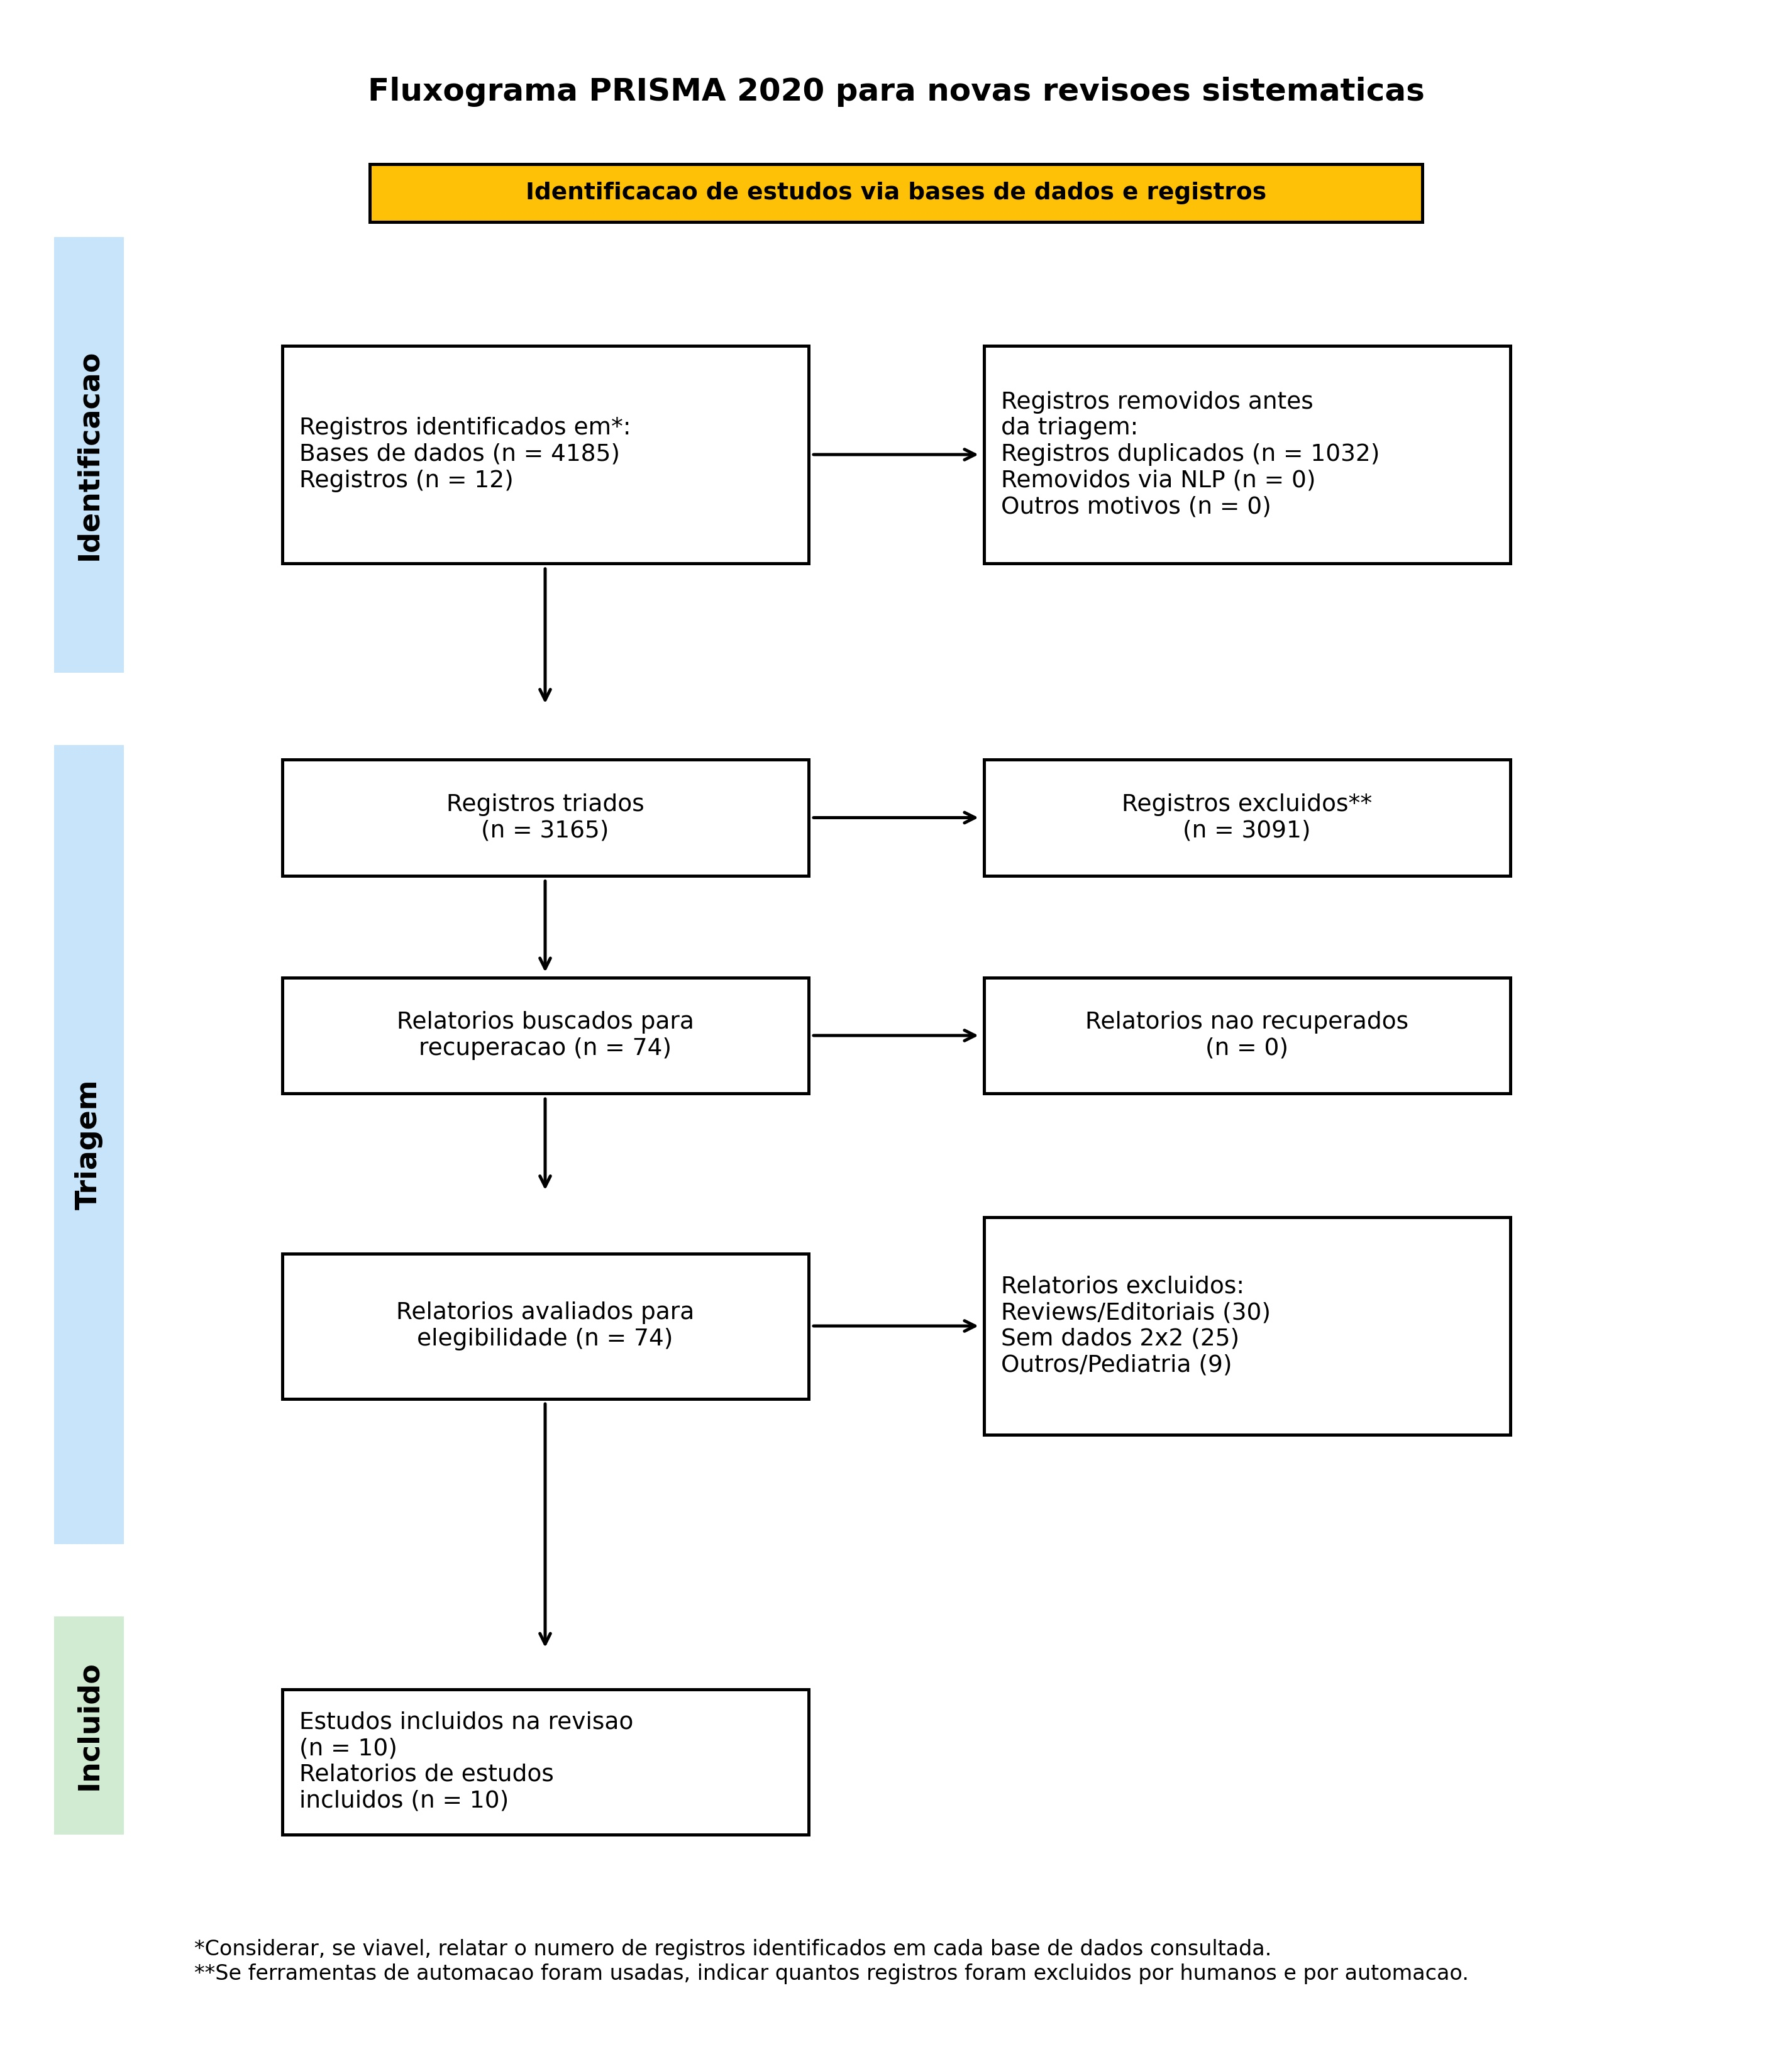
\includegraphics[width=0.85\textwidth]{figures/Fig8_PRISMA_Flowchart_V10.jpg}
    \vspace{4pt}
    \begin{singlespace}
    \centering\small Fonte: Elaborado pelo autor (2026).
    \end{singlespace}
\end{figure}

\begin{table}[H]
\centering
\caption{Características dos Estudos Bivariados Incluídos (N=9)}
\label{tab:estudos}
\resizebox{\textwidth}{!}{
\begin{tabular}{lllrrrrr}
\toprule
Estudo & Classe do modelo & Cenário Clínico & N Total & VP & FP & FN & VN \\
\midrule
Hong 2025a \cite{hong2025a} & Domínio-esp. & Pneumotórax & 2.145 & 181 & 142 & 9 & 1.813 \\
Hong 2025b \cite{hong2025b} & Domínio-esp. & Triagem de Tuberculose & 800 & 360 & 56 & 18 & 366 \\
Ostrovsky 2025 \cite{ostrovsky} & Propósito geral & Pneumonia vs. Normal & 1.400 & 141 & 77 & 44 & 1.138 \\
Huang 2023 \cite{huang2023} & Domínio-esp. & Raio X Emergência & 500 & 139 & 5 & 25 & 331 \\
Huang 2025 \cite{huang2025} & Domínio-esp. & Pneumotórax (Prospective) & 97.651 & 24 & 22 & 9 & 97.596 \\
Akçay 2025 \cite{akcay} & Propósito geral & Pneumotórax (spontaneous) & 220 & 78 & 4 & 32 & 106 \\
Ciflik 2026 \cite{ciflik} & Propósito geral & Pneumotórax (real-world) & 240 & 30 & 18 & 0 & 192 \\
Güzel 2026 \cite{guzel} & Propósito geral & Pneumotórax (SIIM-ACR) & 10.675 & 523 & 415 & 1.856 & 7.881 \\
Khovanova 2026 \cite{khovanova} & Propósito geral & Nódulo Pulmonar & 83 & 12 & 3 & 26 & 42 \\
\bottomrule
\end{tabular}
}
\begin{singlespace}
\centering\small Fonte: Elaborado pelo autor (2026), com base nos estudos primários citados.
\end{singlespace}
\end{table}

O desempenho de acurácia diagnóstica estimado de forma individual para cada estudo primário é detalhado na Tabela \ref{tab:desempenho}, evidenciando elevada dispersão dos resultados, com a sensibilidade individual variando de 22,0\% a 100,0\% e a especificidade de 86,7\% a 100,0\%.

\begin{table}[H]
\centering
\caption{Desempenho Diagnóstico Individual dos Estudos}
\label{tab:desempenho}
\begin{tabular}{lcrrrrrr}
\toprule
Estudo & Sensibilidade & Especificidade & VP & FP & FN & VN & Acurácia \\
\midrule
Hong 2025a & 95,3\% & 92,7\% & 181 & 142 & 9 & 1.813 & 93,0\% \\
Hong 2025b & 95,2\% & 86,7\% & 360 & 56 & 18 & 366 & 90,8\% \\
Ostrovsky 2025 & 76,2\% & 93,7\% & 141 & 77 & 44 & 1.138 & 91,4\% \\
Huang 2023 & 84,8\% & 98,5\% & 139 & 5 & 25 & 331 & 94,0\% \\
Huang 2025 & 72,7\% & 100,0\% & 24 & 22 & 9 & 97.596 & 100,0\% \\
Akçay 2025 & 70,9\% & 96,4\% & 78 & 4 & 32 & 106 & 83,6\% \\
Ciflik 2026 & 100,0\% & 91,4\% & 30 & 18 & 0 & 192 & 92,5\% \\
Güzel 2026 & 22,0\% & 95,0\% & 523 & 415 & 1.856 & 7.881 & 78,7\% \\
Khovanova 2026 & 31,6\% & 93,3\% & 12 & 3 & 26 & 42 & 65,1\% \\
\bottomrule
\end{tabular}
\begin{singlespace}
\centering\small Fonte: Elaborado pelo autor (2026), com base nos estudos primários citados.
\end{singlespace}
\end{table}

A avaliação do risco de viés e preocupações com a aplicabilidade pelo instrumento QUADAS-2 está resumida na Tabela \ref{tab:quadas2}. Os estudos Akçay 2025 \cite{akcay} e Khovanova 2026 \cite{khovanova} foram julgados com alto risco de viés no domínio ``Seleção de Pacientes'' por adotarem desenhos caso-controle balanceados que induzem viés de espectro e não refletem a prevalência clínica real. Sete estudos apresentaram risco incerto no domínio ``Teste Índice'' pela ausência de thresholds de corte textuais declarados de forma unívoca em seus métodos de prompt. A distribuição detalhada das avaliações de risco de viés e preocupações de aplicabilidade para cada estudo primário individual pode ser visualizada na Figura \ref{fig:quadas_traffic}, e o resumo geral das avaliações por domínio está ilustrado na Figura \ref{fig:quadas_summary}.

\begin{table}[H]
\centering
\caption{Avaliação da Qualidade Metodológica dos Estudos pelo Instrumento QUADAS-2 (N=12)}
\label{tab:quadas2}
\resizebox{\textwidth}{!}{
\begin{tabular}{lccccccc}
\toprule
 & \multicolumn{4}{c}{Risco de Viés} & \multicolumn{3}{c}{Preocupações com Aplicabilidade} \\
\cmidrule(r){2-5} \cmidrule(l){6-8}
Estudo & Seleção & Teste Índice & Padrão Ref. & Fluxo/Tempo & Seleção & Teste Índice & Padrão Ref. \\
\midrule
Hong 2025a & Baixo & Baixo & Baixo & Baixo & Baixo & Baixo & Baixo \\
Hong 2025b & Baixo & Baixo & Baixo & Baixo & Baixo & Baixo & Baixo \\
Ostrovsky 2025 & Baixo & Incerto & Baixo & Baixo & Baixo & Baixo & Baixo \\
Huang 2023 & Baixo & Incerto & Baixo & Baixo & Baixo & Baixo & Baixo \\
Huang 2025 & Baixo & Incerto & Baixo & Baixo & Baixo & Baixo & Baixo \\
Akçay 2025 & Alto & Incerto & Baixo & Baixo & Baixo & Baixo & Baixo \\
Ciflik 2026 & Baixo & Incerto & Baixo & Baixo & Baixo & Baixo & Baixo \\
Lee 2025 & Baixo & Baixo & Incerto & Baixo & Baixo & Baixo & Baixo \\
Güzel 2026 & Incerto & Baixo & Baixo & Baixo & Baixo & Baixo & Baixo \\
Khovanova 2026 & Alto & Incerto & Baixo & Incerto & Baixo & Baixo & Baixo \\
Bai 2026 & Incerto & Baixo & Baixo & Baixo & Baixo & Baixo & Baixo \\
Bulut 2025 & Incerto & Incerto & Baixo & Alto & Baixo & Baixo & Baixo \\
\bottomrule
\end{tabular}
}
\begin{singlespace}
\centering\small Fonte: Elaborado pelo autor (2026).
\end{singlespace}
\end{table}

\begin{figure}[H]
    \centering
    \caption{QUADAS-2: Avaliação Individual por Estudo e Domínio.}
    \label{fig:quadas_traffic}
    \vspace{4pt}
    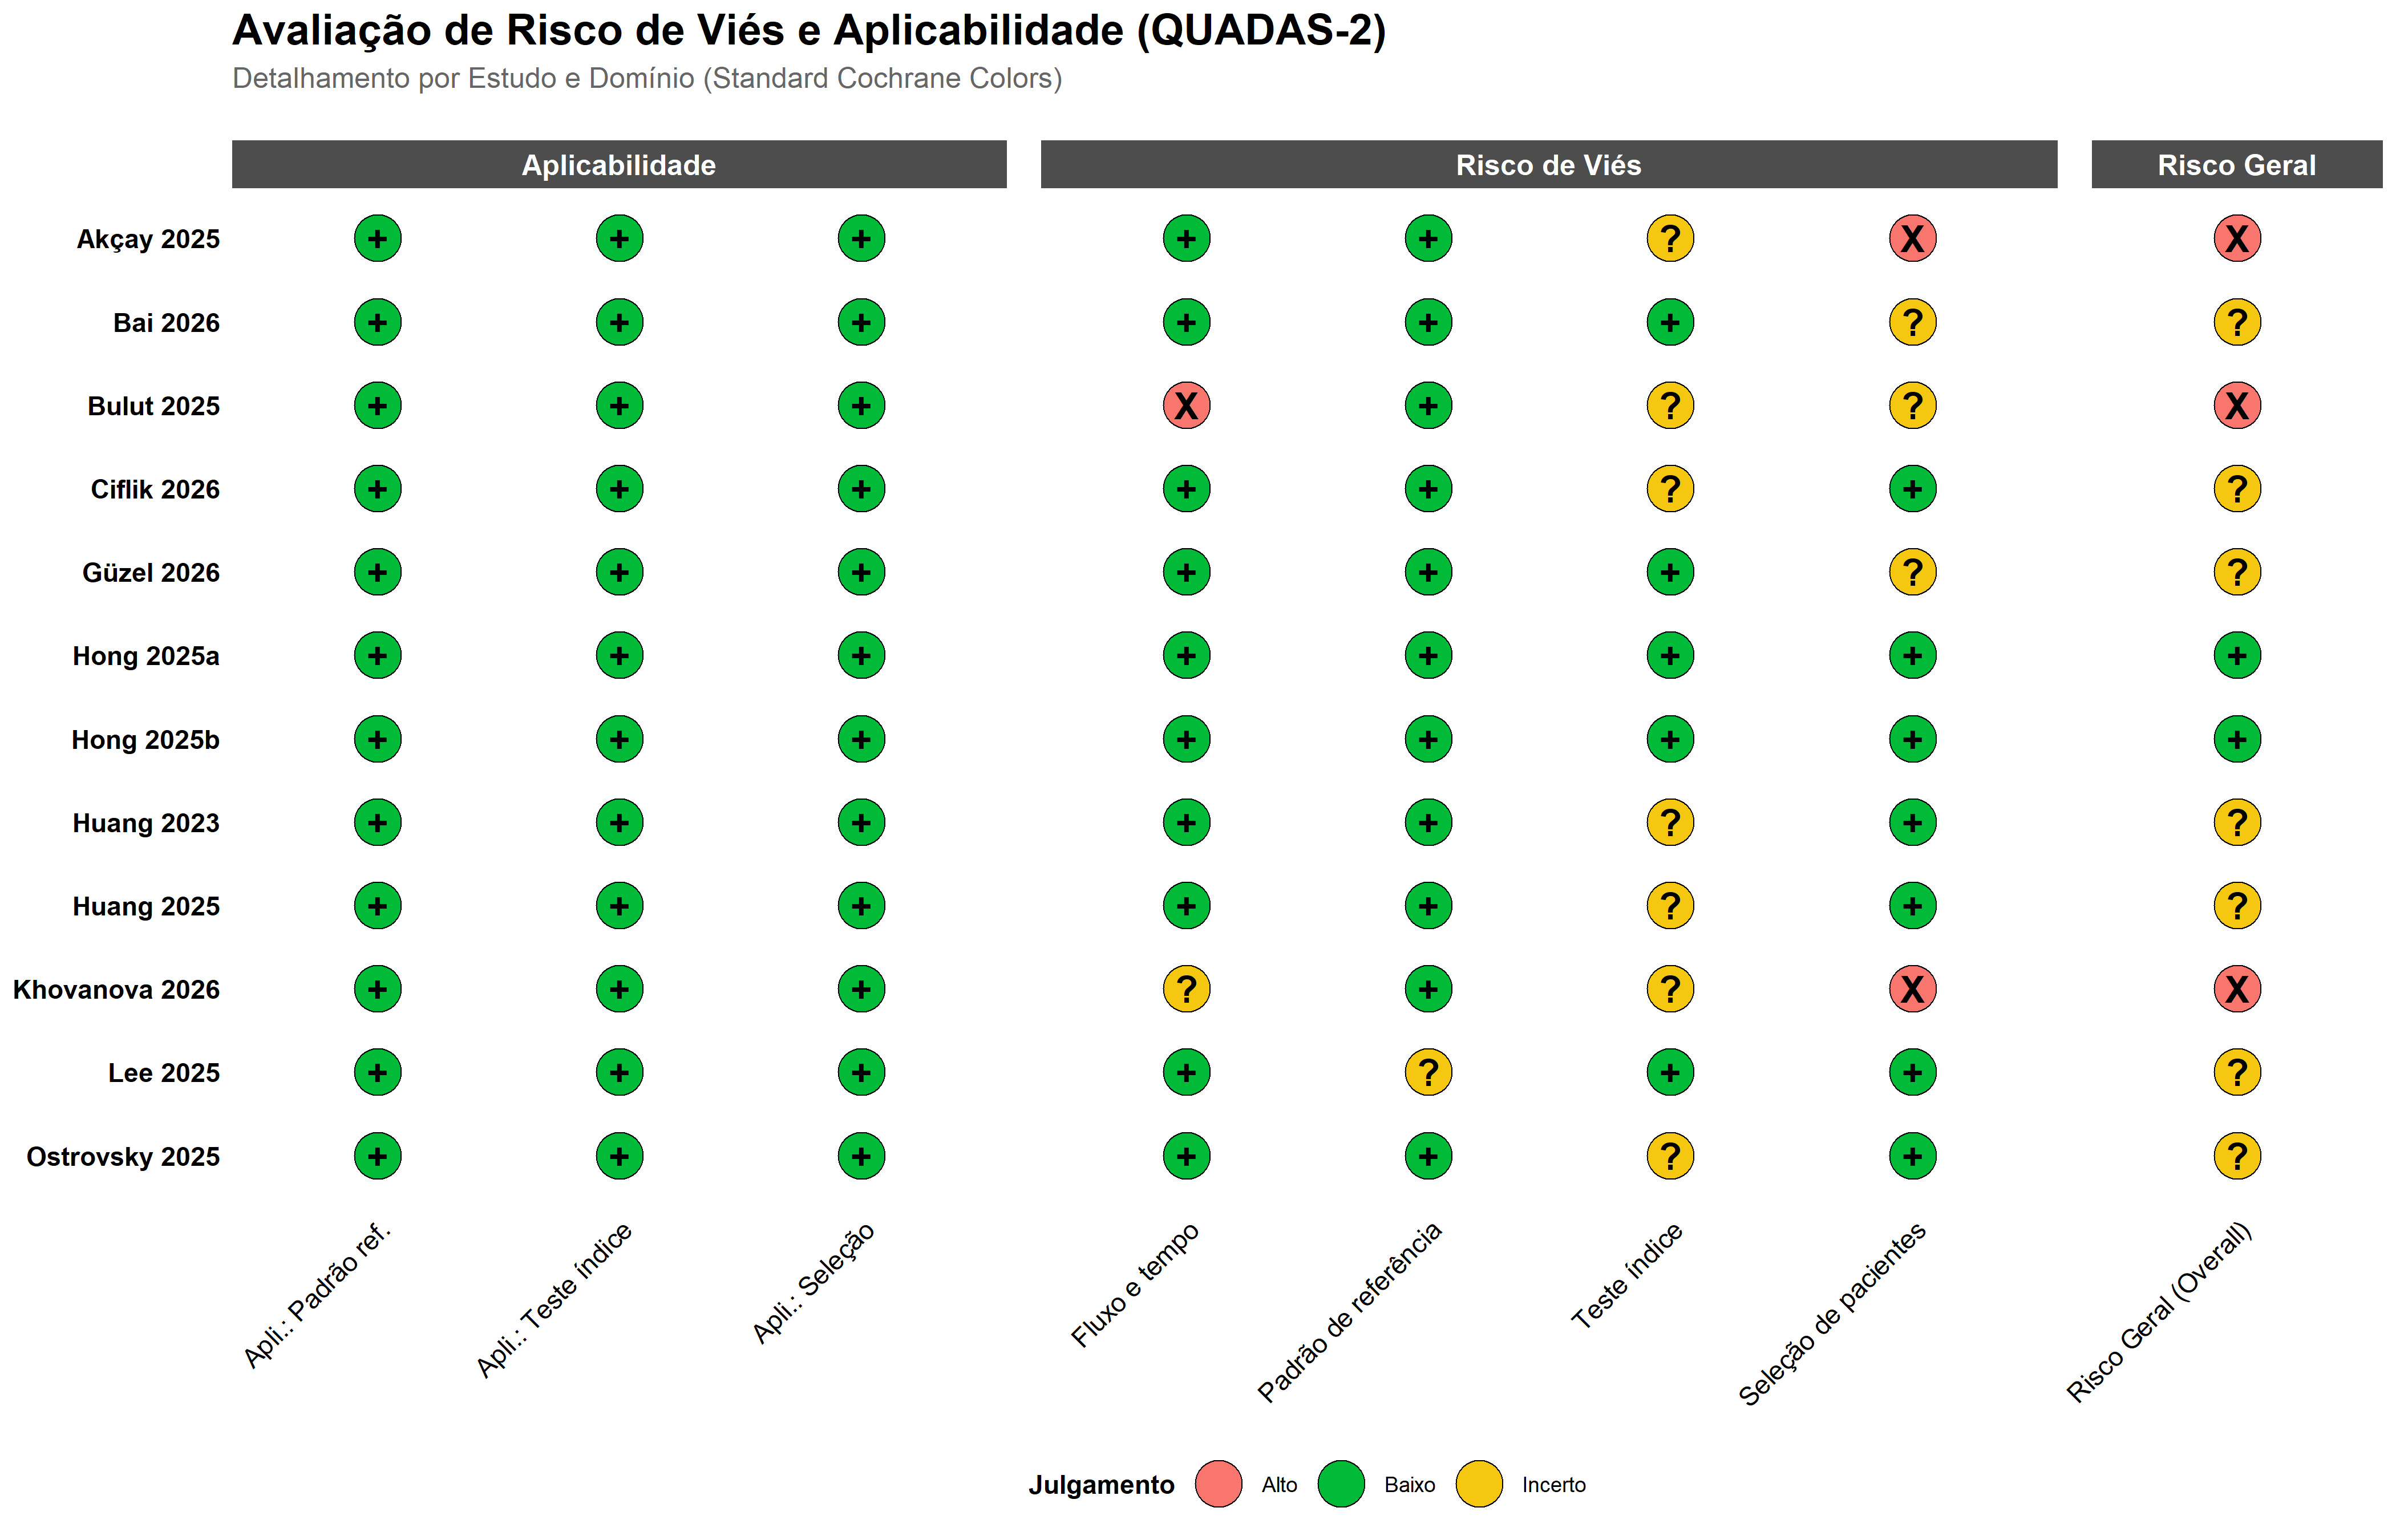
\includegraphics[width=0.9\textwidth]{figures/Grafico_QUADAS2_TrafficLight.jpg}
    \vspace{4pt}
    \begin{singlespace}
    \centering\small Fonte: Elaborado pelo autor (2026).
    \end{singlespace}
\end{figure}

\begin{figure}[H]
    \centering
    \caption{QUADAS-2: Resumo por Domínio (N=12).}
    \label{fig:quadas_summary}
    \vspace{4pt}
    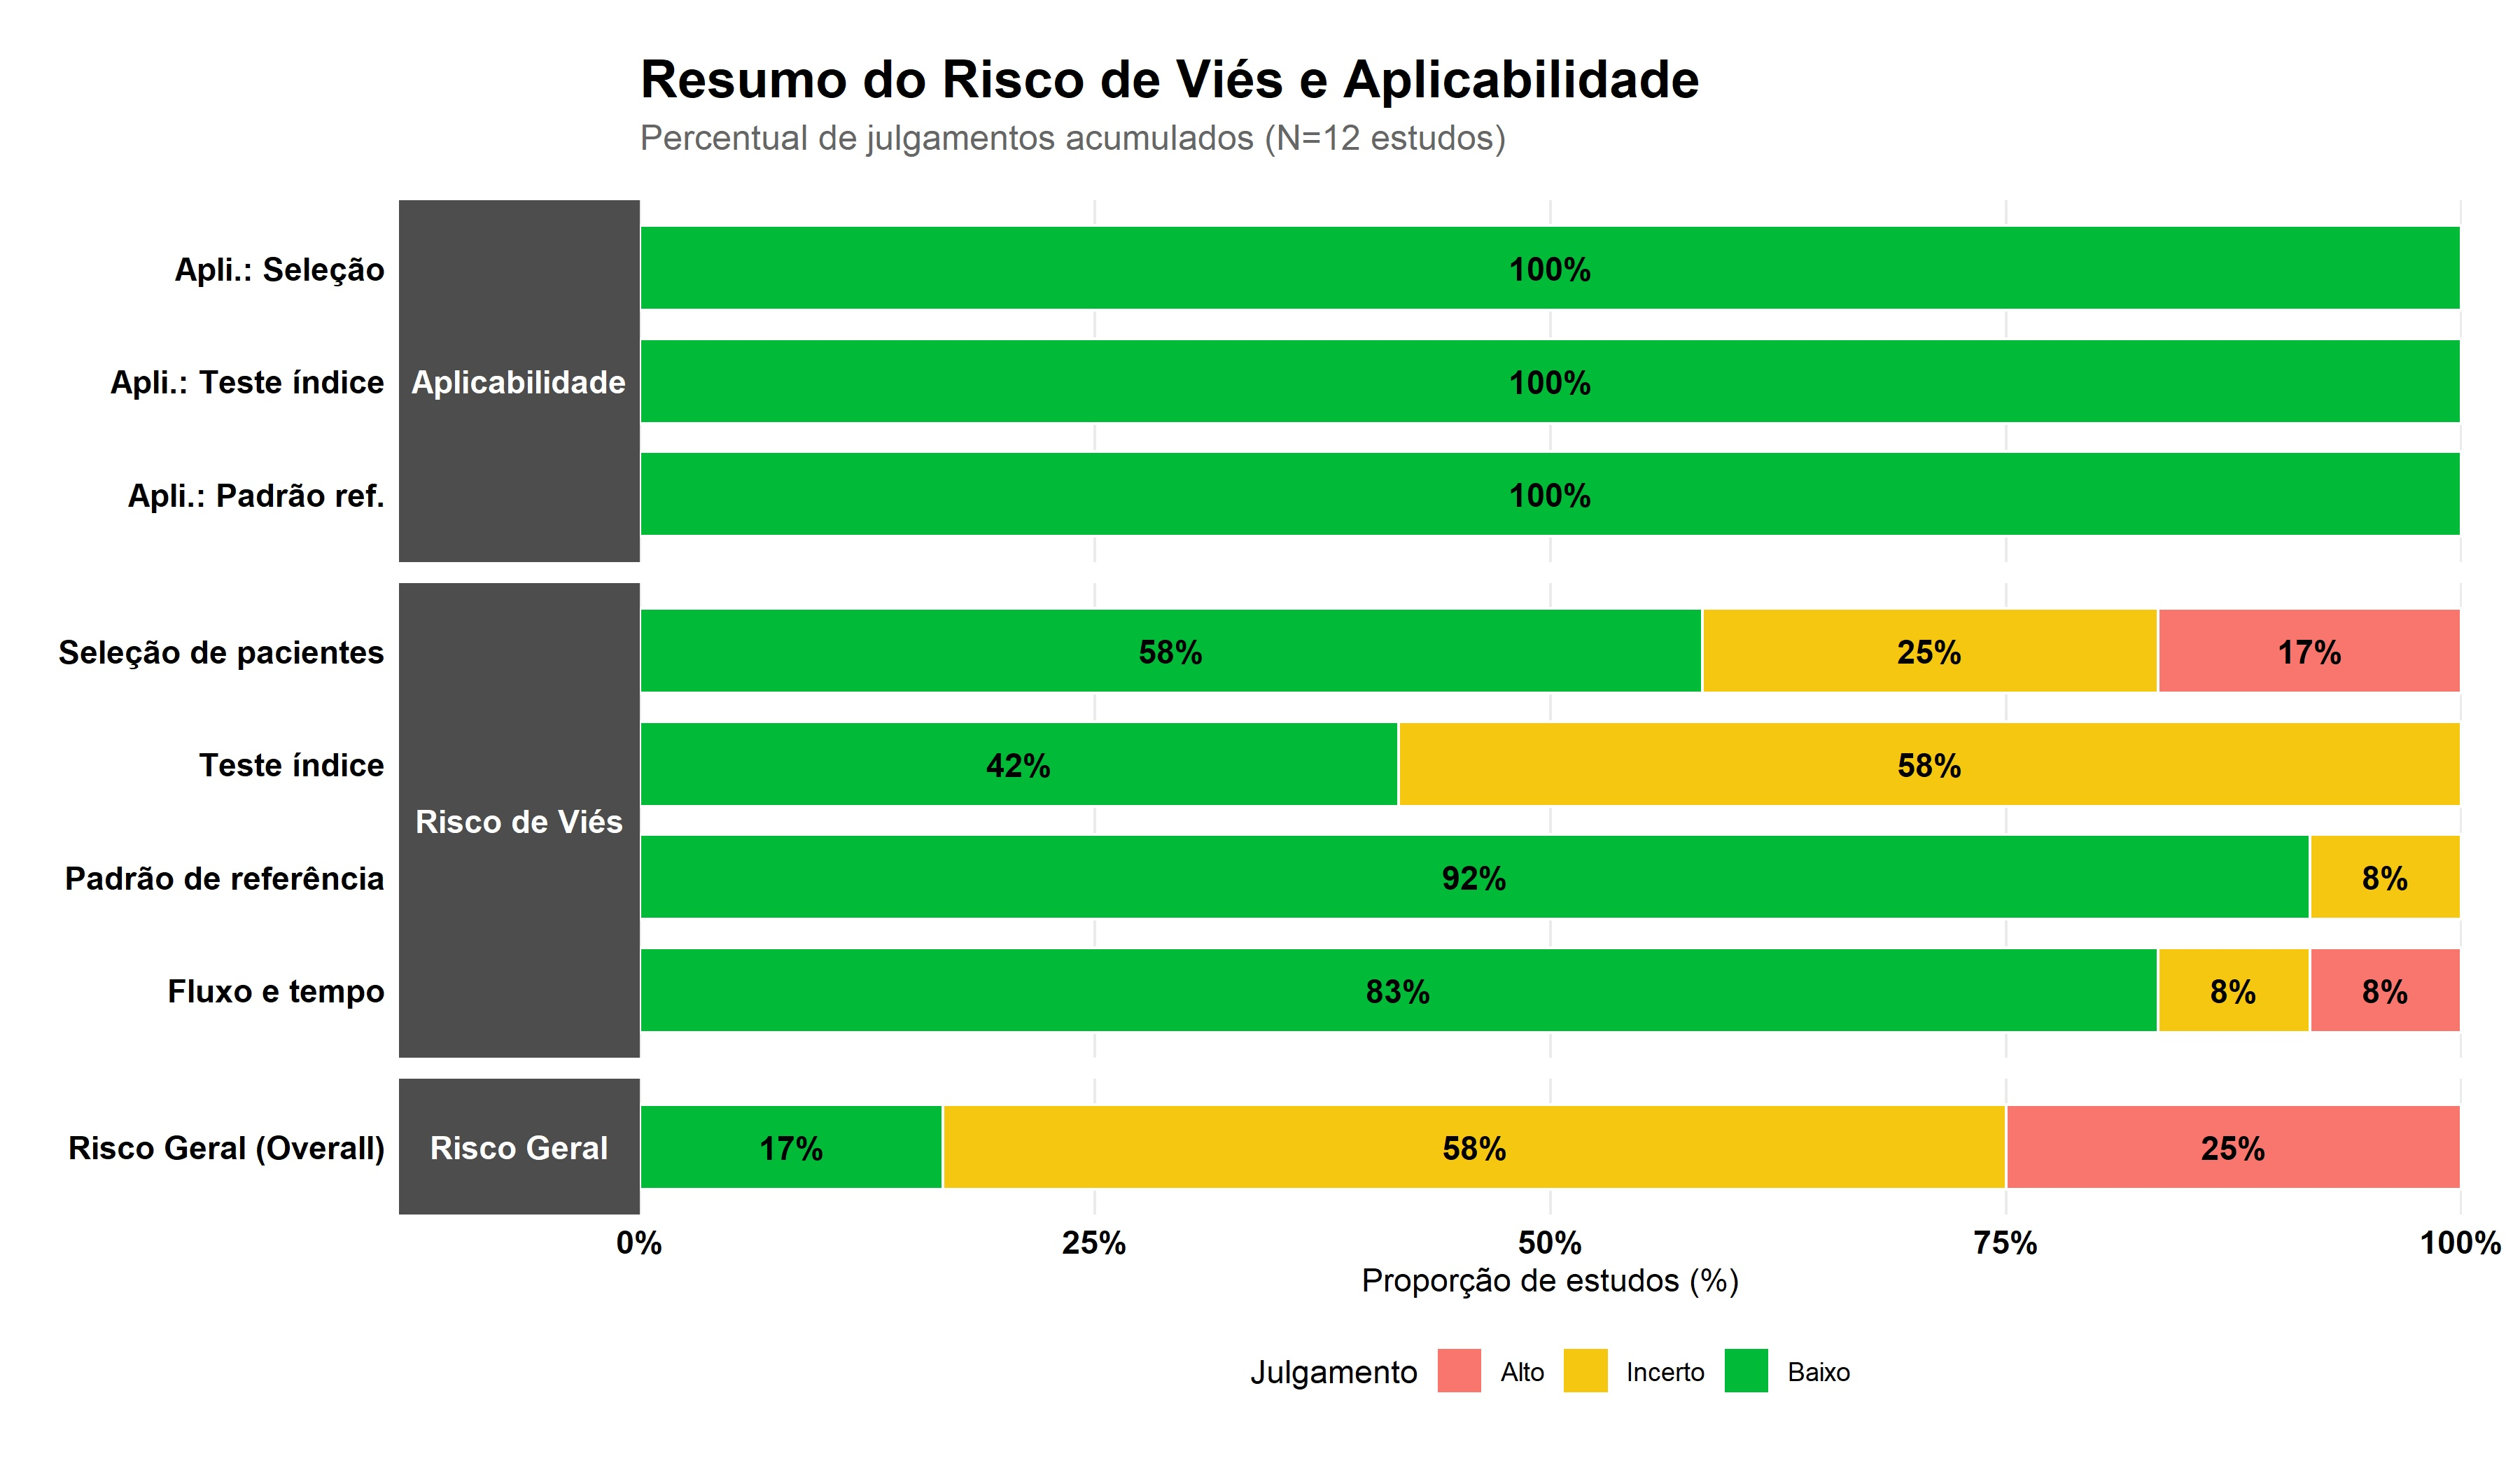
\includegraphics[width=0.9\textwidth]{figures/Grafico_QUADAS2_Summary.jpg}
    \vspace{4pt}
    \begin{singlespace}
    \centering\small Fonte: Elaborado pelo autor (2026).
    \end{singlespace}
\end{figure}

\subsection{Meta-análise Exploratória: Pool Principal (N=9)}
A síntese quantitativa das estimativas de acurácia diagnóstica do pool principal bivariado de N=9 estudos (113.714 exames) é apresentada na Tabela \ref{tab:agrupados}. O modelo bivariado estimou uma sensibilidade agrupada de 78,1\% (IC 95\%: 54,9--91,3\%) e uma especificidade agrupada de 96,8\% (IC 95\%: 89,1--99,1\%). A Razão de Verossimilhança Positiva (RV+) foi estimada em 24,10, enquanto a Razão de Verossimilhança Negativa (RV-) foi de 0,226. A área sob a curva (AUC) SROC foi calculada em 0,953. As estimativas individuais e a sensibilidade agrupada de efeitos aleatórios são apresentadas no Forest Plot da Figura \ref{fig:forest_sens}. De forma análoga, a dispersão das especificidades individuais e a especificidade agrupada correspondente estão ilustradas no Forest Plot da Figura \ref{fig:forest_spec}. A curva SROC (Summary Receiver Operating Characteristic) hierárquica e suas respectivas regiões de confiança e predição são exibidas na Figura \ref{fig:sroc}.

\begin{table}[H]
\centering
\caption{Resultados Meta-analíticos Agrupados do Pool Principal (N=9)}
\label{tab:agrupados}
\begin{tabular}{lcc}
\toprule
Métrica & Estimativa & Intervalo de Confiança (IC 95\%) \\
\midrule
Sensibilidade Agrupada & 78,1\% & 54,9\%--91,3\% \\
Especificidade Agrupada & 96,8\% & 89,1\%--99,1\% \\
Razão de Verossimilhança Positiva (RV+) & 24,10 & --- \\
Razão de Verossimilhança Negativa (RV-) & 0,226 & --- \\
Estudos Incluídos & 9 & --- \\
Total de Participantes & 113.714 & --- \\
\bottomrule
\end{tabular}
\begin{singlespace}
\centering\small Fonte: Elaborado pelo autor (2026), com base no modelo bivariado de Reitsma, método REML.
\end{singlespace}
\end{table}

O intervalo de predição de 95\% estimado para a sensibilidade foi de 6,4\% a 99,5\%, enquanto para a especificidade variou de 18,1\% a 100,0\% ($\tau_{\text{sens}}=1,583$; $\tau_{\text{fpr}}=1,966$). A elevada amplitude dos intervalos de predição evidencia a alta variabilidade e heterogeneidade intrínseca do desempenho de leitura visual entre os diferentes modelos avaliados no pool, indicando que não é possível assegurar um patamar fixo de acurácia diagnóstica em novos ambientes sem controle rigoroso dos modelos.

\begin{figure}[H]
    \centering
    \caption{Forest Plot da Sensibilidade Agrupada (N=9, Raw 2$\times$2).}
    \label{fig:forest_sens}
    \vspace{4pt}
    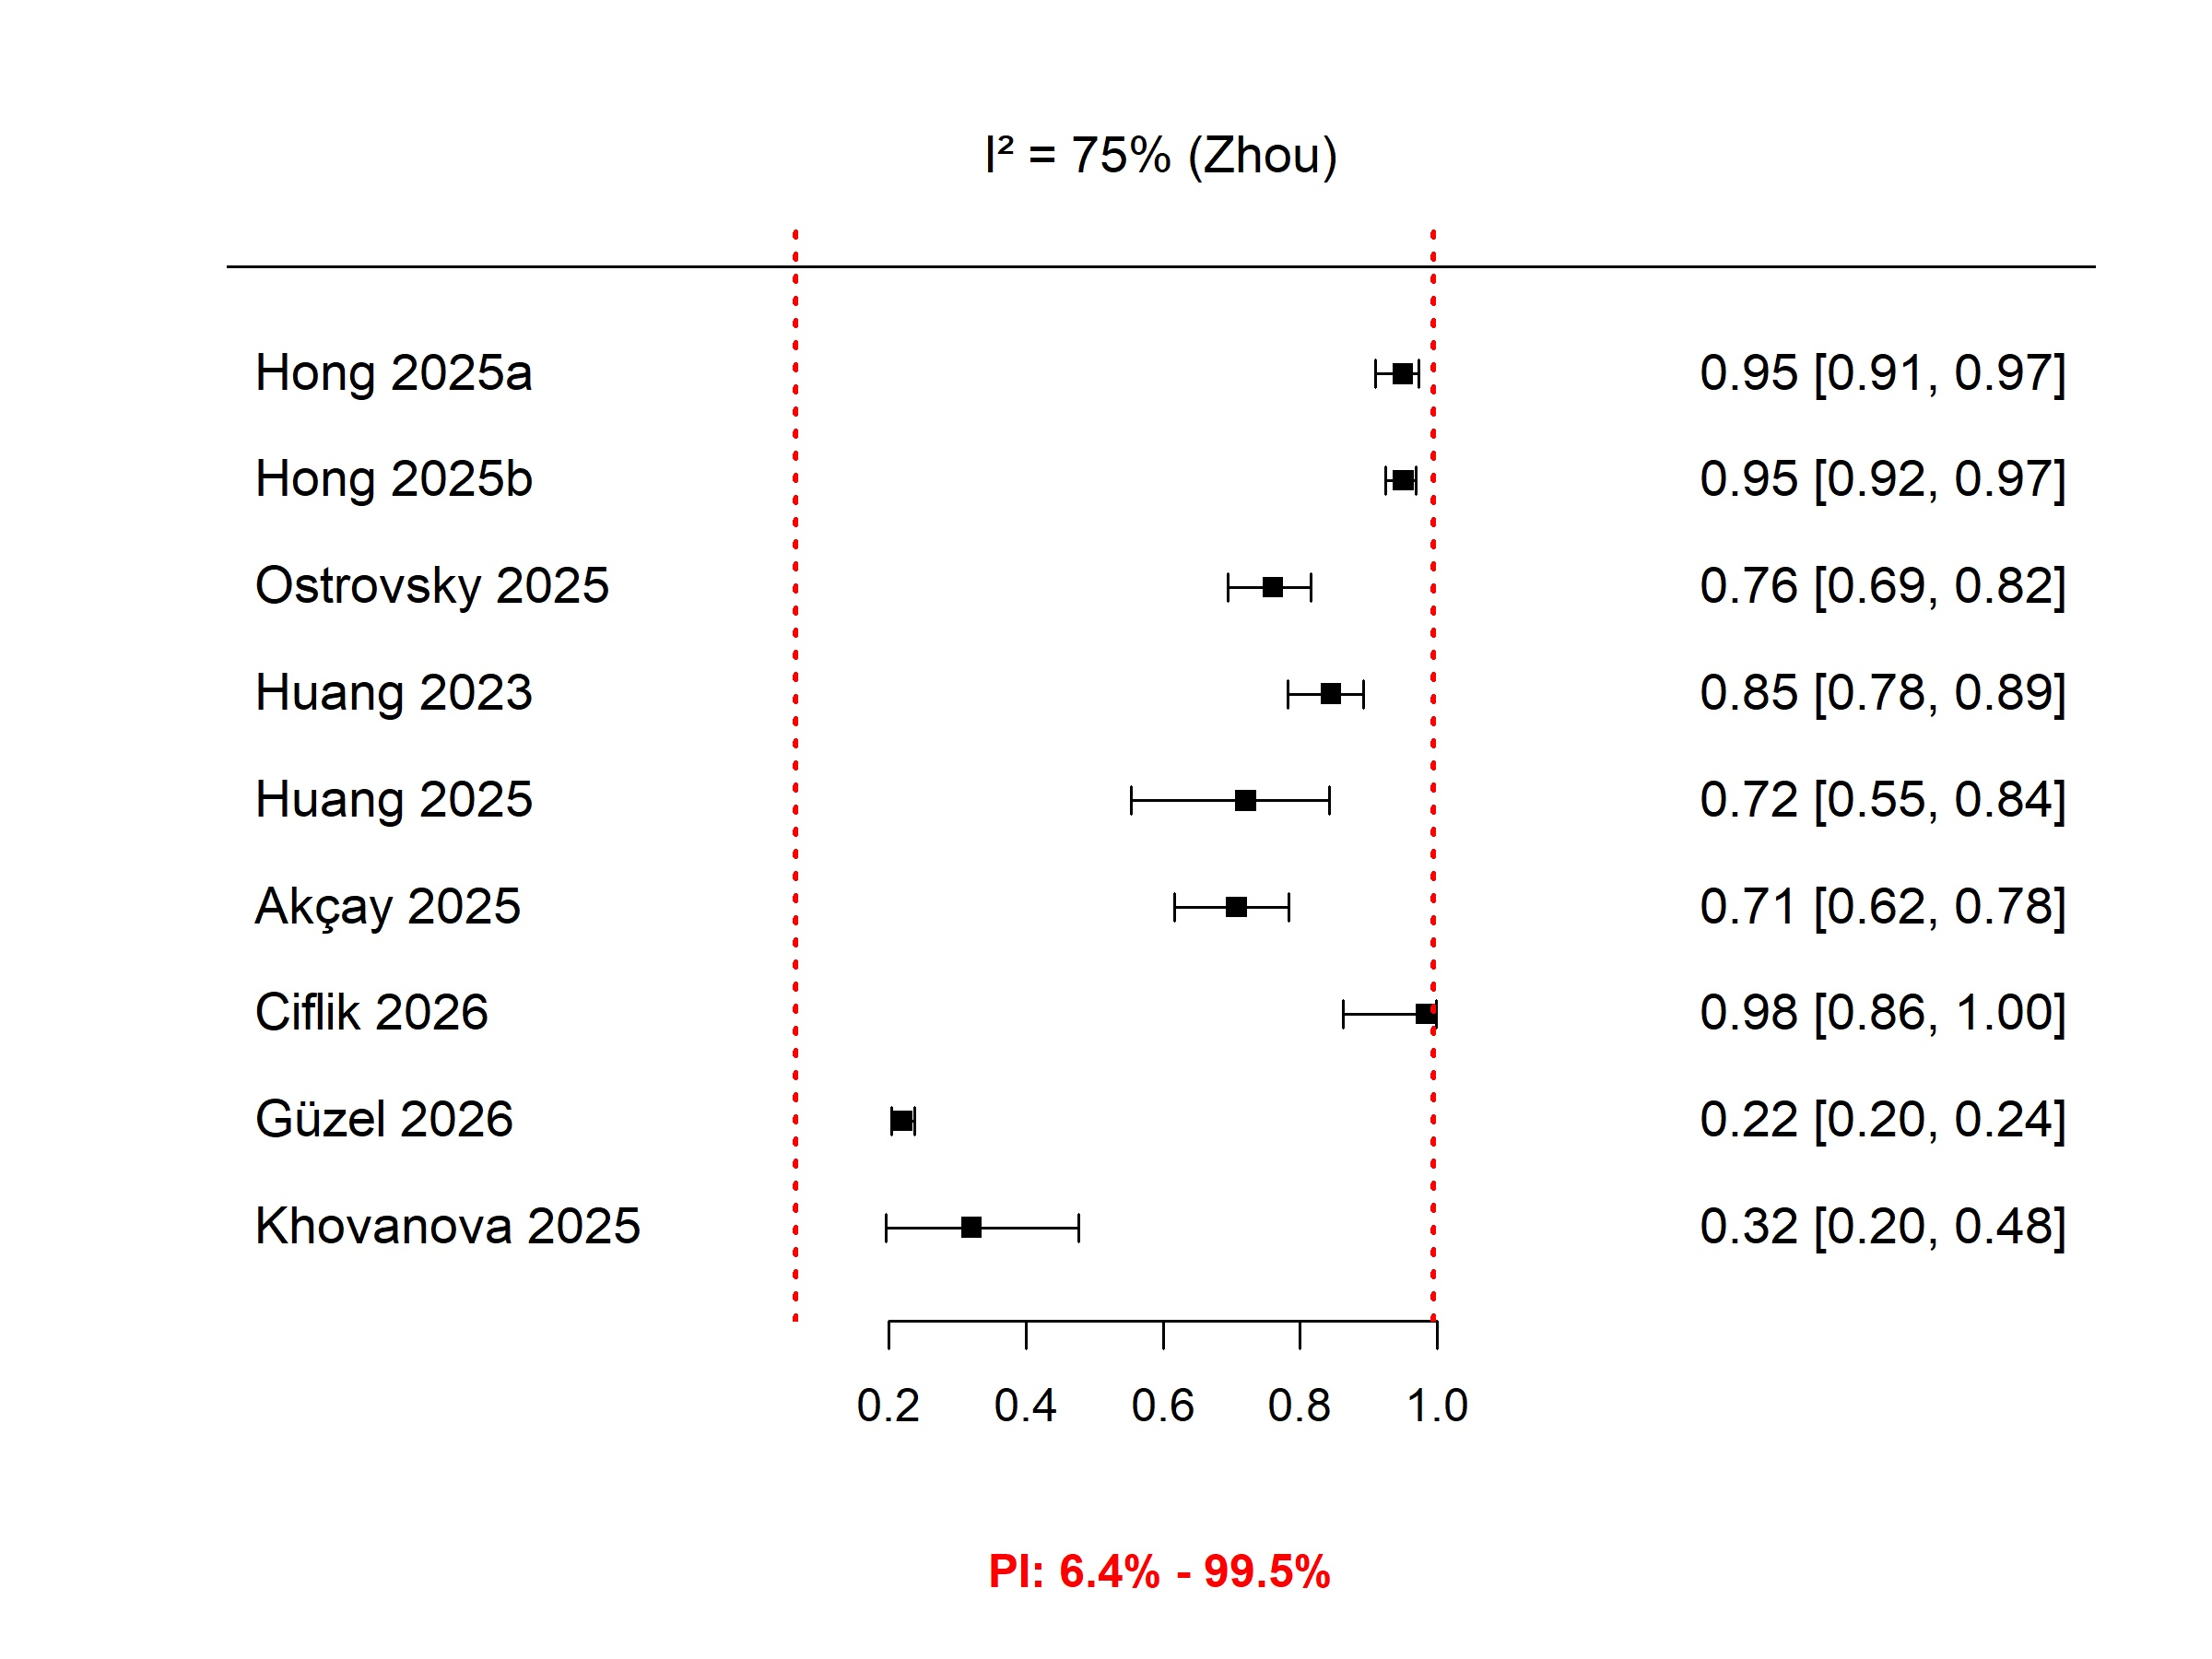
\includegraphics[width=0.85\textwidth]{figures/Fig1_Forest_Sens_V10.jpg}
    \vspace{4pt}
    \begin{singlespace}
    \centering\small Fonte: Elaborado pelo autor (2026).
    \end{singlespace}
\end{figure}

\begin{figure}[H]
    \centering
    \caption{Forest Plot da Especificidade Agrupada (N=9, Raw 2$\times$2).}
    \label{fig:forest_spec}
    \vspace{4pt}
    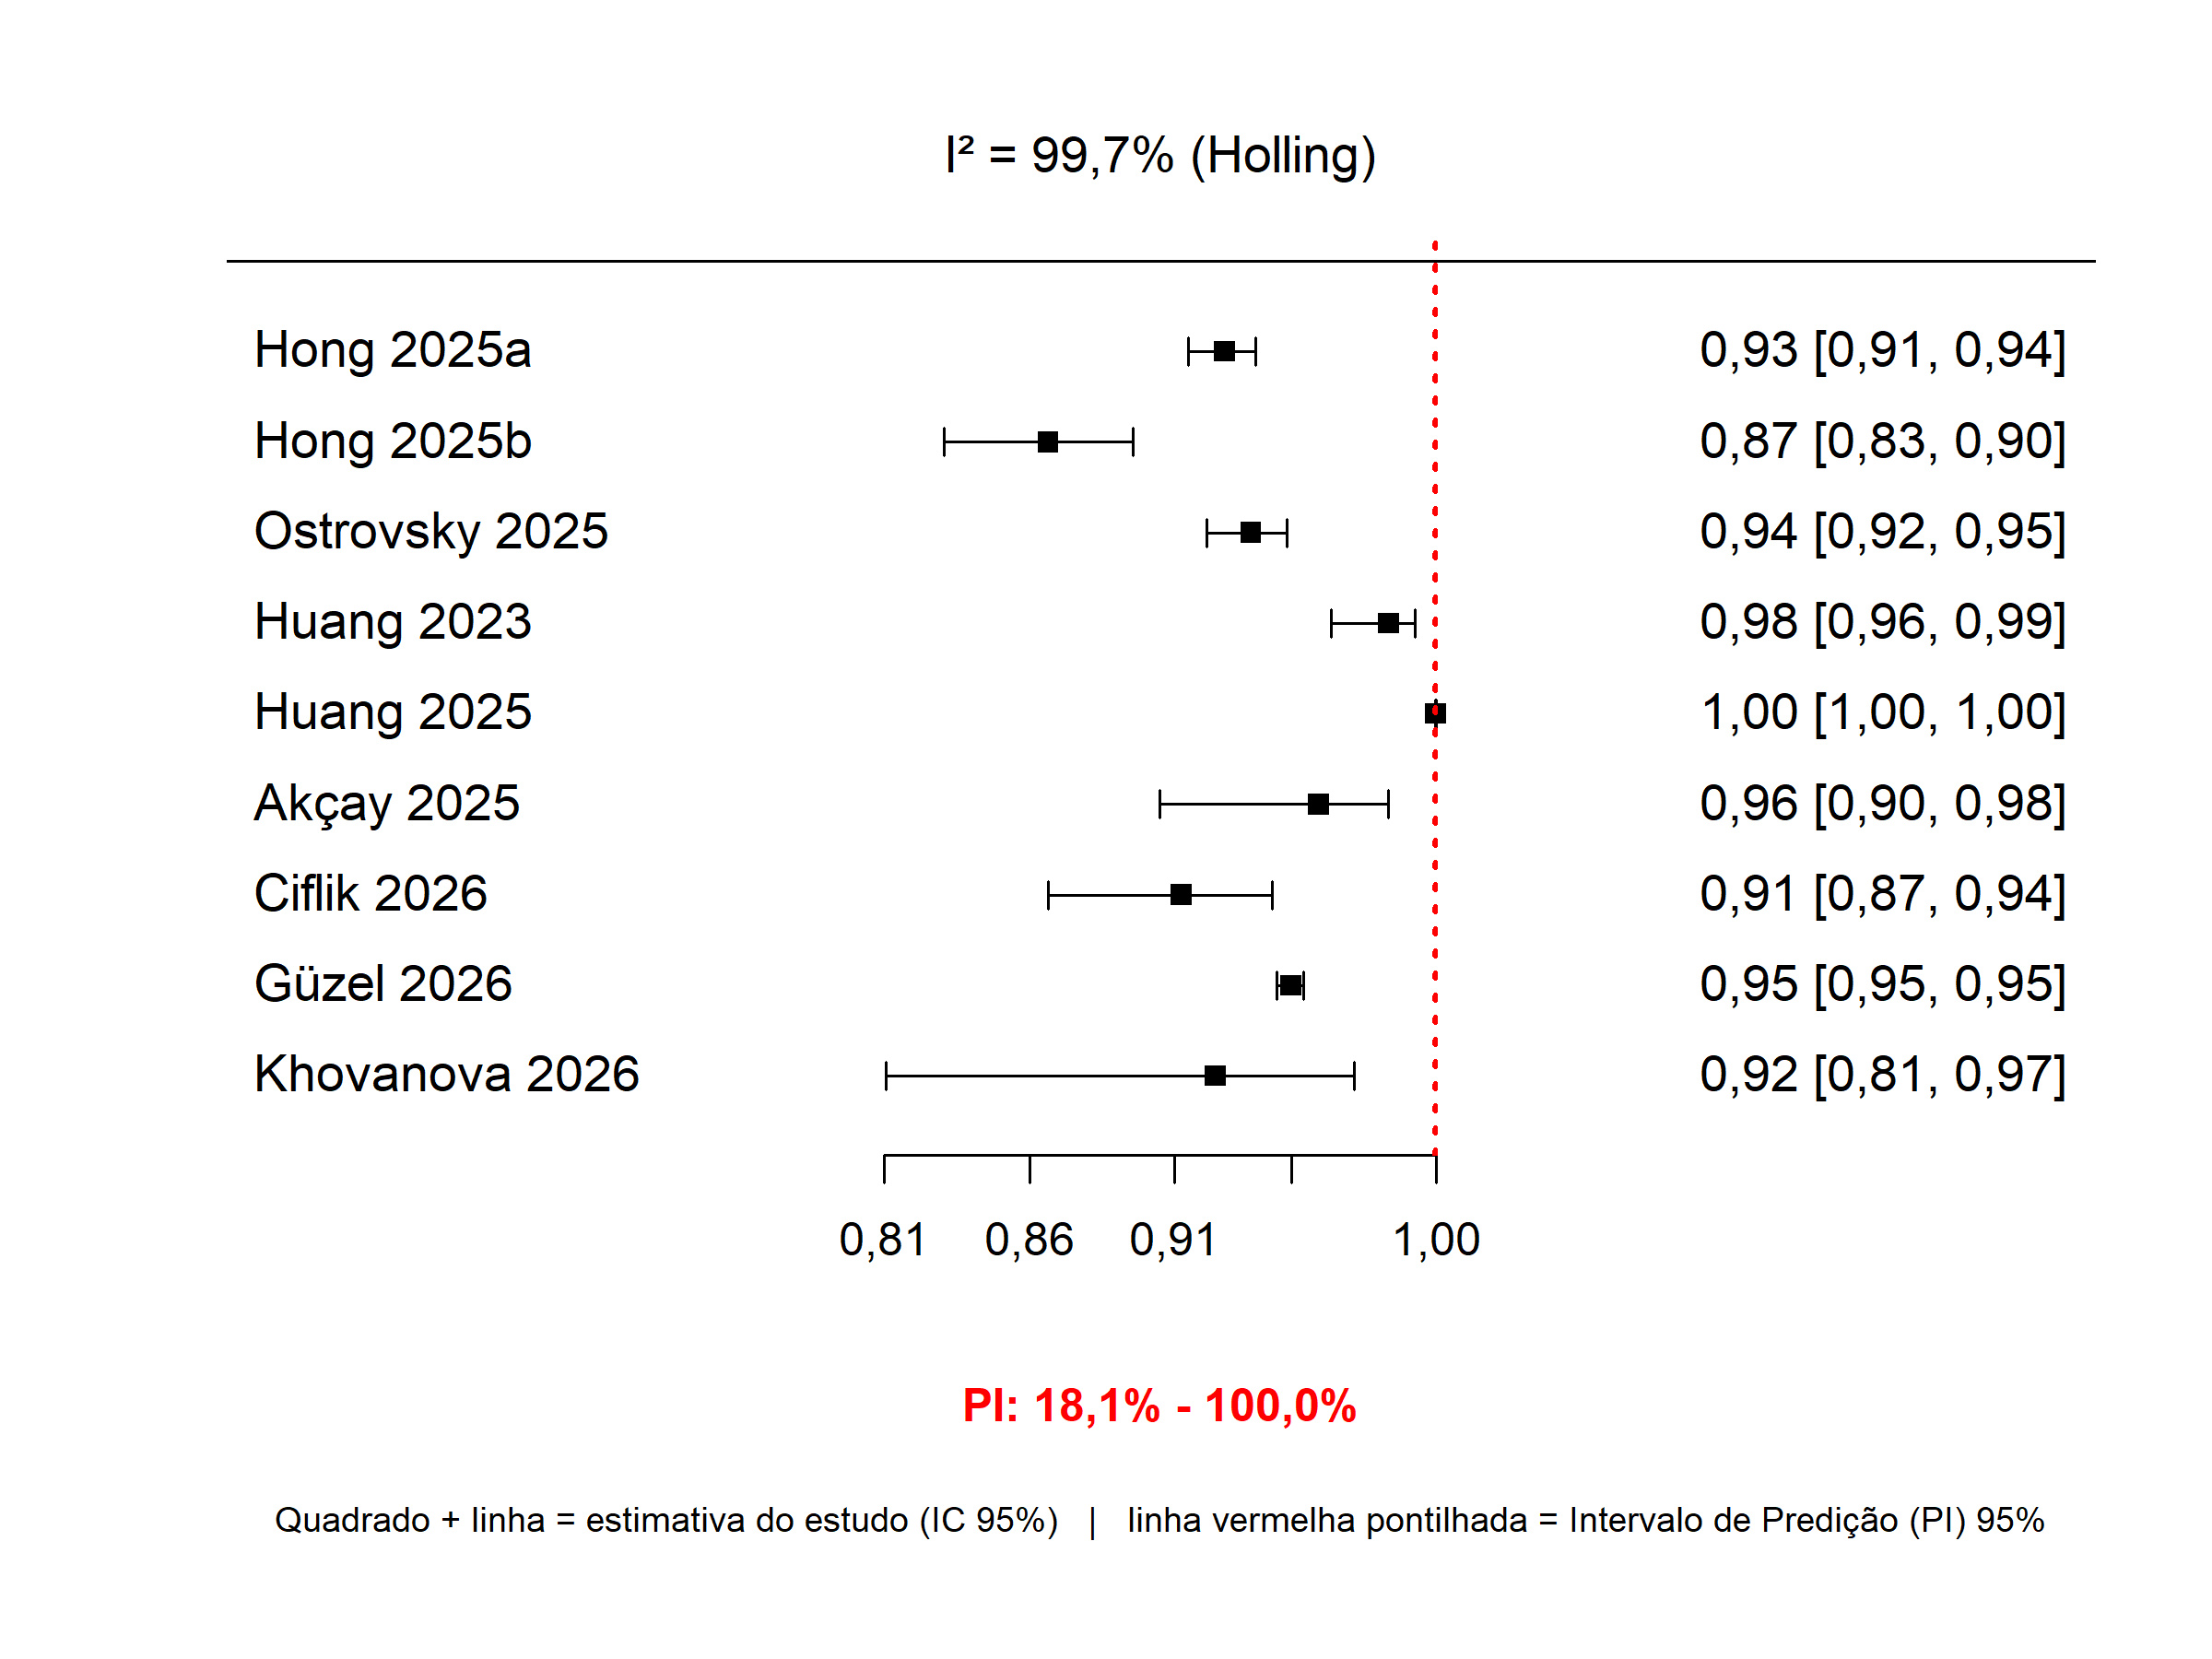
\includegraphics[width=0.85\textwidth]{figures/Fig2_Forest_Spec_V10.jpg}
    \vspace{4pt}
    \begin{singlespace}
    \centering\small Fonte: Elaborado pelo autor (2026).
    \end{singlespace}
\end{figure}

\begin{figure}[H]
    \centering
    \caption{Curva SROC Hierárquica e Regiões de Confiança e Predição: Pool Principal (N=9).}
    \label{fig:sroc}
    \vspace{4pt}
    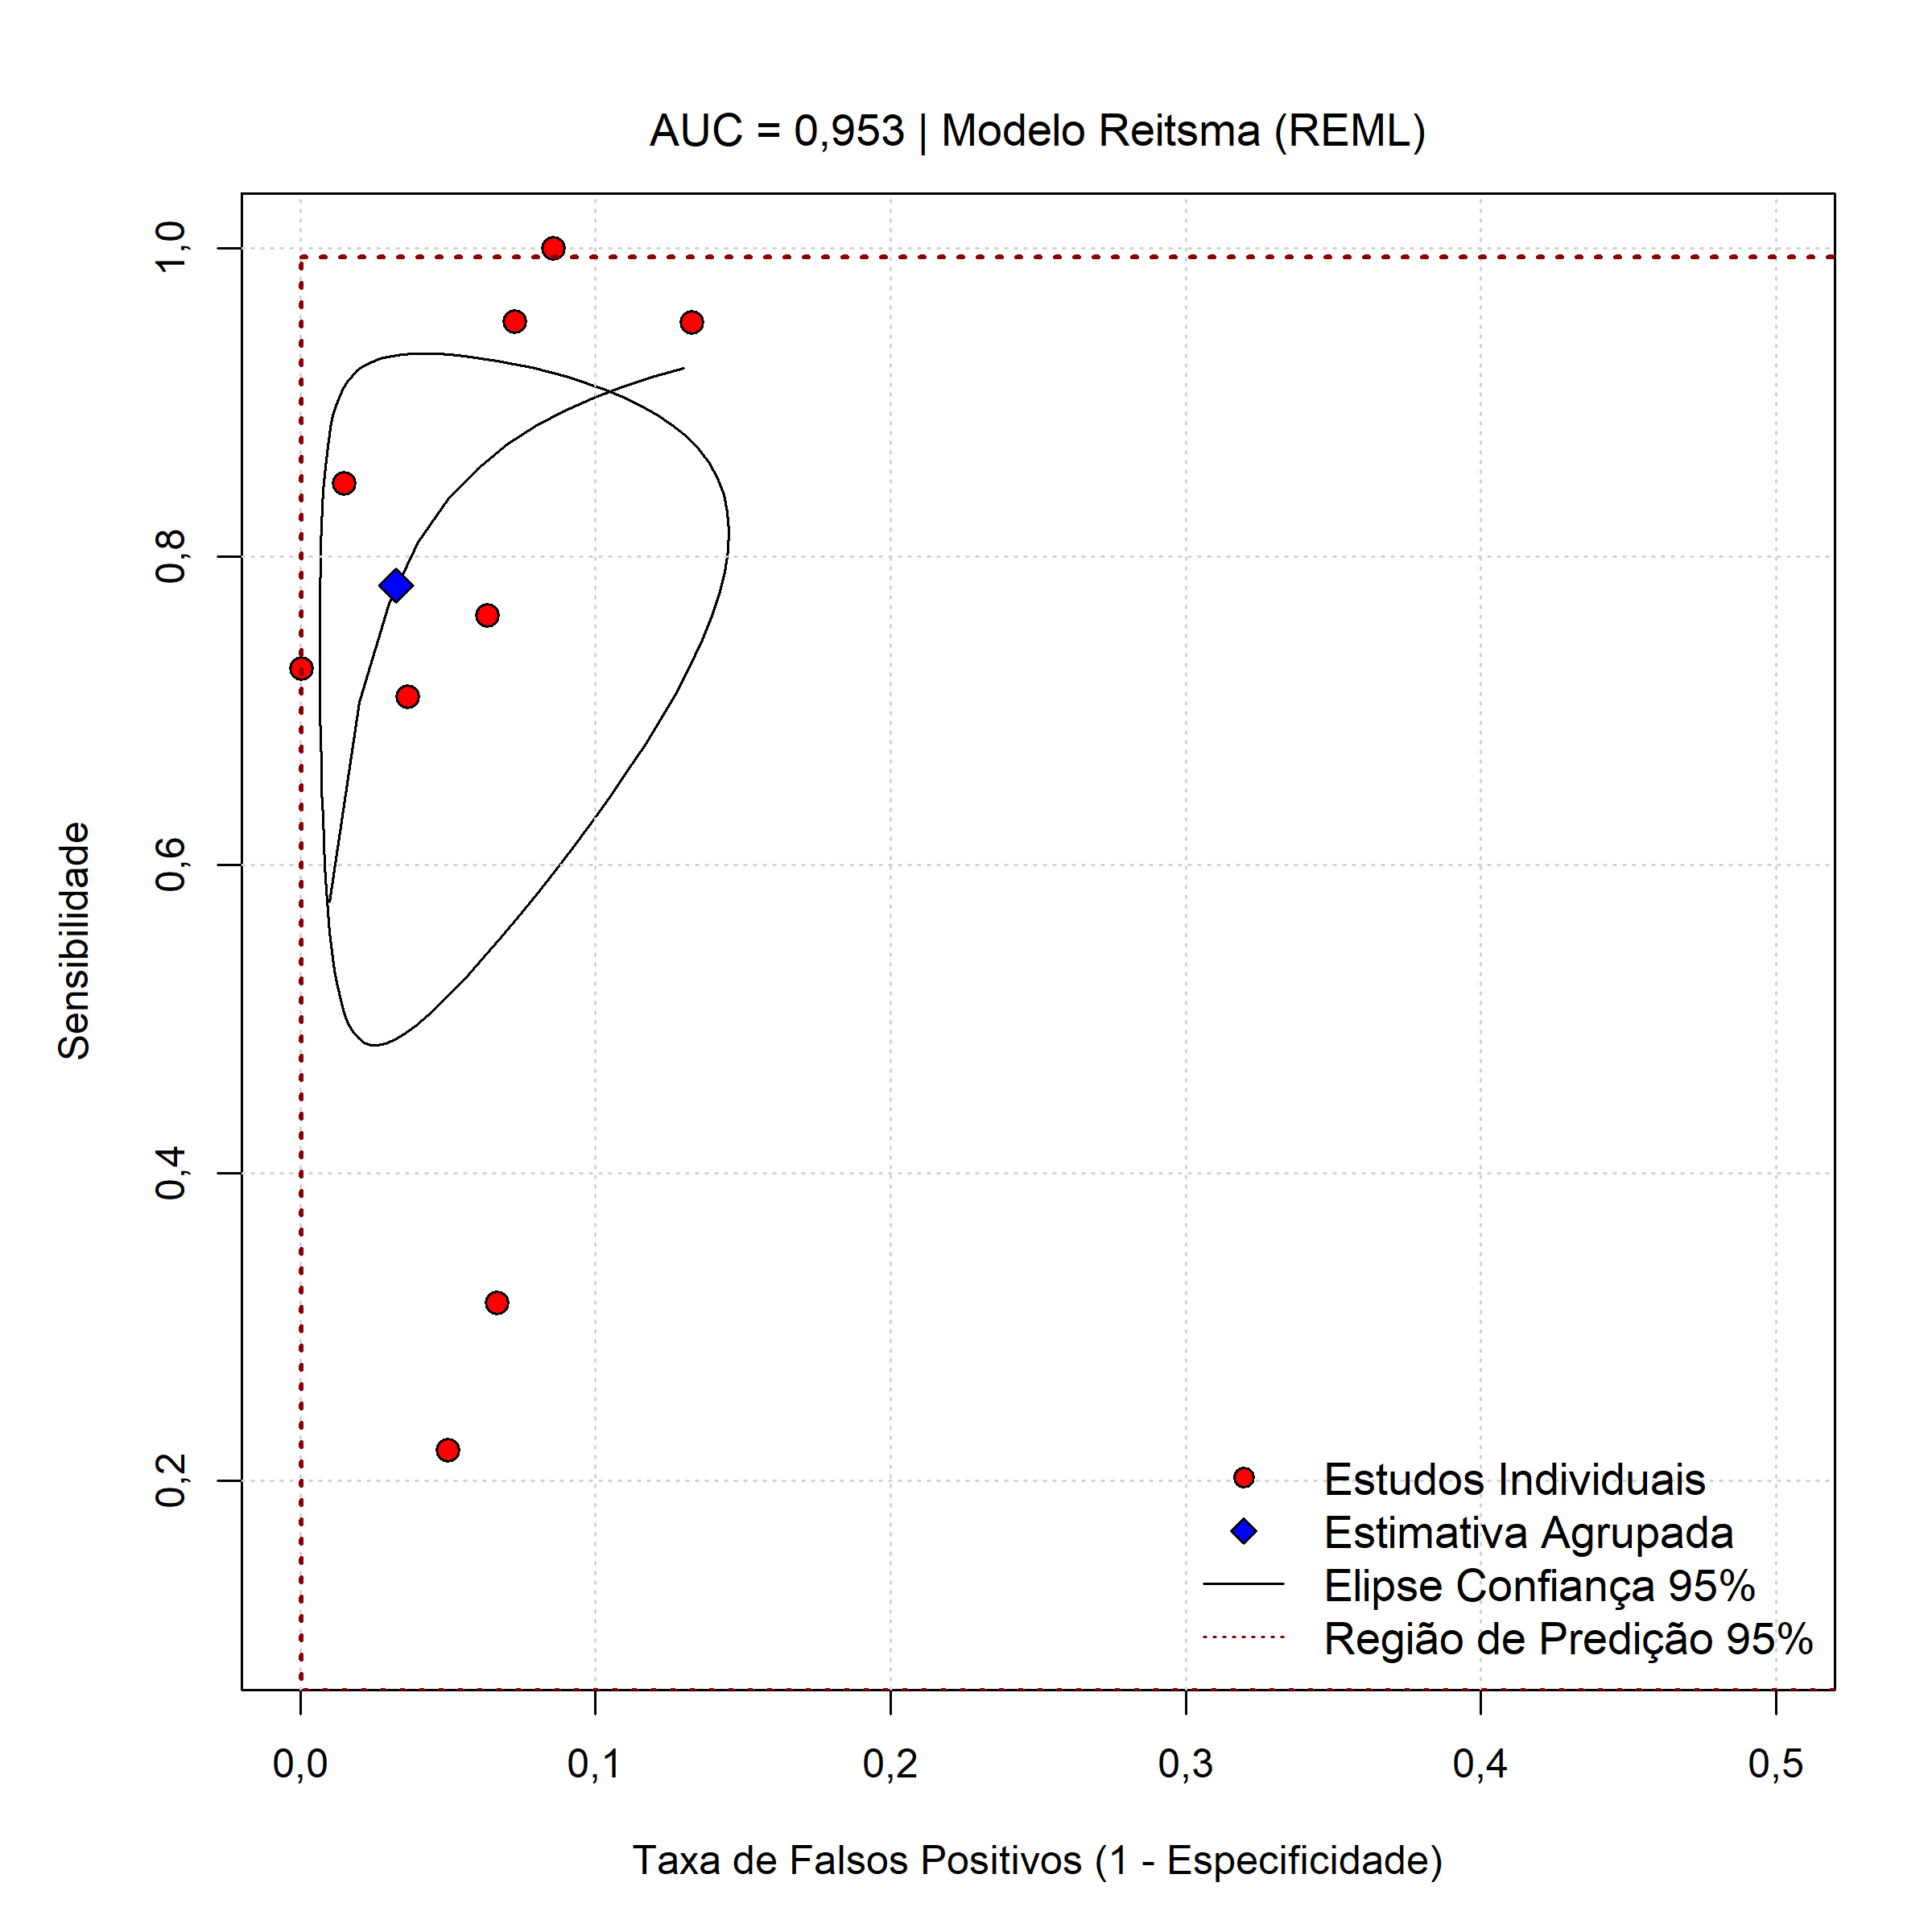
\includegraphics[width=0.85\textwidth]{figures/Fig4_SROC_Prediction_V10.jpg}
    \vspace{4pt}
    \begin{singlespace}
    \centering\small Fonte: Elaborado pelo autor (2026).
    \end{singlespace}
\end{figure}

\subsection{Análises de Sensibilidade}
As análises de sensibilidade executadas para avaliar a robustez das estimativas do ponto sumário são sumarizadas na Tabela \ref{tab:sensibilidade}.

\begin{table}[H]
\centering
\caption{Resultados das Análises de Sensibilidade (Robustez)}
\label{tab:sensibilidade}
\resizebox{\textwidth}{!}{
\begin{tabular}{lcrrcccrcc}
\toprule
Cenário & Estudos (N) & Participantes & Sens (\%) & IC 95\% & Spec (\%) & IC 95\% & RV+ & RV- & AUC \\
\midrule
1. Pool completo (N=9) & 9 & 113.714 & 78,1 & 54,9--91,3 & 96,8 & 89,1--99,1 & 24,10 & 0,226 & 0,953 \\
A. Sem Güzel 2026 & 8 & 103.039 & 83,1 & 65,3--92,7 & 97,0 & 88,0--99,3 & 27,28 & 0,175 & 0,954 \\
B. Sem Huang 2025 & 8 & 16.063 & 79,2 & 52,8--92,8 & 93,7 & 91,0--95,6 & 12,54 & 0,222 & 0,950 \\
C. Sem Ambos & 7 & 5.388 & 84,6 & 64,8--94,3 & 93,7 & 90,2--96,0 & 13,41 & 0,164 & 0,958 \\
D. Sem Alto Risco & 7 & 113.411 & 83,7 & 59,4--94,8 & 97,2 & 86,8--99,5 & 29,83 & 0,167 & 0,963 \\
E. Subgrupo PTX & 5 & 110.931 & 79,0 & 40,0--95,5 & 98,0 & 83,8--99,8 & 38,87 & 0,214 & 0,962 \\
\bottomrule
\end{tabular}
}
\begin{singlespace}
\centering\small Fonte: Elaborado pelo autor (2026).
\end{singlespace}
\end{table}

A exclusão de Güzel 2026 (Cenário A) elevou a sensibilidade agrupada para 83,1\% (IC 95\%: 65,3--92,7\%), demonstrando o forte efeito deste estudo de baixa sensibilidade diagnóstica sobre o pool geral. 

A exclusão de Huang 2025 (Cenário B) reduziu a especificidade agrupada de 96,8\% para 93,7\% (IC 95\%: 91,0--95,6\%), o que comprova que a especificidade próxima a 100\% do pool principal era artificialmente inflada pelo peso amostral maciço (N=97.651) e baixa prevalência de doença deste estudo.

A exclusão simultânea de ambos os extremos (Cenário C) resultou em sensibilidade de 84,6\% e especificidade de 93,7\%. Este cenário, contudo, remove também o estudo de pior desempenho (Güzel 2026), deslocando a sensibilidade para cima; por essa razão, adota-se o Cenário B --- e não o C --- como referência para a leitura clínica (Seção 4.2), por ser o recorte que corrige a distorção de especificidade sem descartar a evidência desfavorável.

\subsection{Heterogeneidade}
A heterogeneidade quantificada pelo índice $I^2$ bivariado de Zhou-Dendukuri foi de 74,6\% no pool principal completo. Pelo método de Holling não ajustado, a variabilidade situou-se entre 89,1\% e 99,7\%, enquanto o método ajustado pelo tamanho amostral situou-se entre 9,1\% e 21,9\%. A acentuada divergência entre as versões ajustada e não ajustada reflete o peso da assimetria amostral do pool, sobretudo a dominância de Huang 2025. A exclusão simultânea dos dois extremos de volume (Cenário C) reduz o índice de Zhou-Dendukuri de 74,6\% para 52,0\%, indicando que parcela relevante --- porém não a totalidade --- da heterogeneidade se associa à dispersão de tamanhos amostrais e prevalências. Ressalte-se, contudo, que a heterogeneidade não diminui em todos os recortes: nos Cenários D (exclusão de estudos com alto risco de viés) e E (subgrupo restrito a pneumotórax), o índice de Zhou-Dendukuri sobe para 86,4\% e 86,6\%, respectivamente. Assim, a variabilidade remanescente não é atribuível apenas ao tamanho amostral e persiste mesmo em subconjuntos clinicamente mais homogêneos, reforçando a leitura de que a inconsistência de desempenho entre modelos e tarefas é intrínseca à literatura primária. A análise do viés de publicação e da assimetria de relato foi realizada graficamente através do Funnel Plot apresentado na Figura \ref{fig:funnel}, complementada pelo teste de regressão de Deeks (p = 0,008), cujo resultado é aqui reportado em caráter estritamente descritivo. Com menos de 10 estudos, o Cochrane-DTA não recomenda a realização nem a interpretação formal desse teste, que carece de poder estatístico adequado; ademais, ele é fortemente sensível à acentuada heterogeneidade de tamanho amostral do pool --- sobretudo ao peso desproporcional de Huang 2025. Por essas razões, o valor obtido não deve ser lido como evidência de viés de publicação, refletindo mais provavelmente um efeito de tamanho de amostra.

\begin{figure}[H]
    \centering
    \caption{Funnel Plot para Avaliação de Viés de Publicação e Assimetria de Relato.}
    \label{fig:funnel}
    \vspace{4pt}
    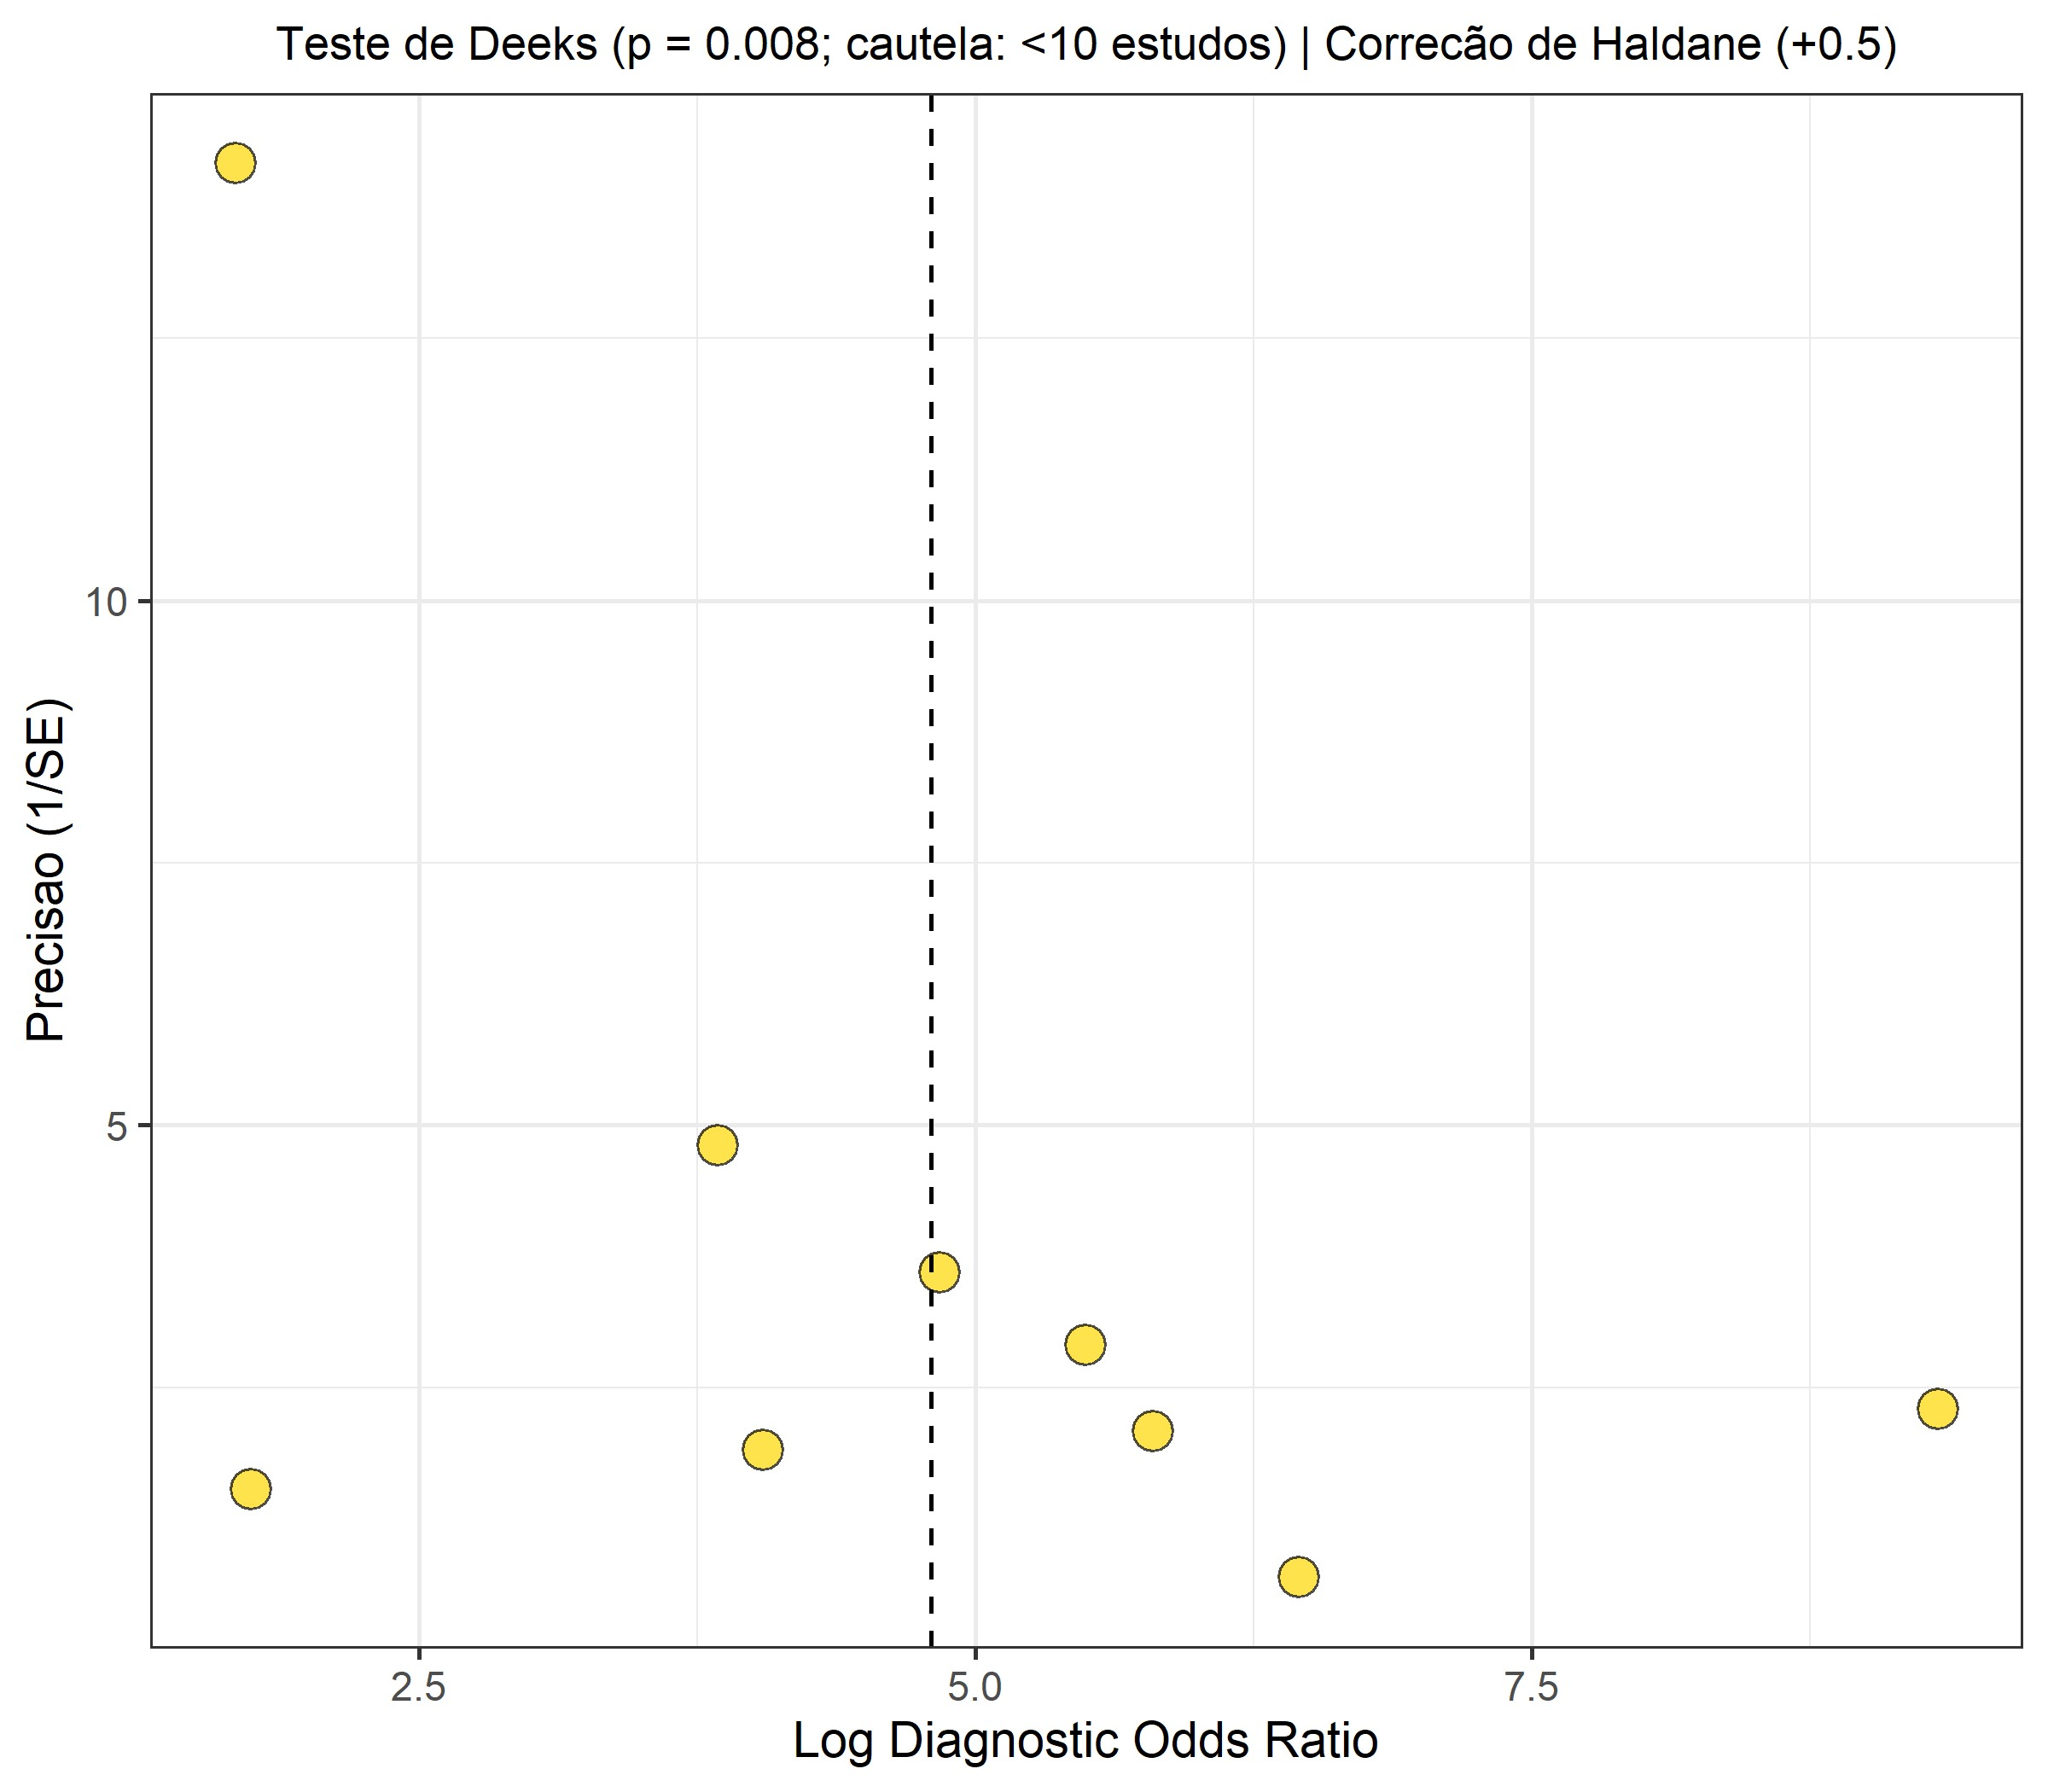
\includegraphics[width=0.85\textwidth]{figures/Fig5_FunnelPlot_V10.jpg}
    \vspace{4pt}
    \begin{singlespace}
    \centering\small Fonte: Elaborado pelo autor (2026).
    \end{singlespace}
\end{figure}

\subsection{Análise Exploratória por Subgrupos}

\subsubsection{Por Especialização do Modelo (Propósito Geral vs. Domínio-específico)}
A comparação de médias aritméticas simples segundo o grau de especialização do modelo-índice (Seção 2.2) revelou o contraste mais nítido de toda a análise exploratória. Os modelos \textbf{domínio-específicos} (N=4 estudos: Hong 2025a, Hong 2025b, Huang 2023 e Huang 2025) alcançaram sensibilidade média de 87,0\% e especificidade média de 94,5\%. Os modelos de \textbf{propósito geral} (N=5 estudos: Ostrovsky 2025, Akçay 2025, Ciflik 2026, Güzel 2026 e Khovanova 2026) obtiveram sensibilidade média de apenas 60,1\%, com especificidade média de 94,0\%, conforme sintetizado na Tabela \ref{tab:subgrupo_arch}. Note-se que a especificidade média é praticamente idêntica entre os grupos (94,5\% vs. 94,0\%), enquanto a sensibilidade difere em cerca de 27 pontos percentuais --- padrão compatível com modelos generalistas que adotam limiares de decisão conservadores. Ressalva-se que a comparação é descritiva: apoia-se em médias não ponderadas e em poucos estudos por braço, não autorizando teste formal de diferença entre grupos.

A baixa sensibilidade média do grupo de propósito geral é fortemente influenciada por Güzel 2026 (22,0\%) e Khovanova 2026 (31,6\%), ambos avaliando modelos comerciais sobre lesões de pequenas dimensões. Em contraste, os modelos adaptados ao domínio radiológico --- notadamente o KARA-CXR nos estudos de Hong --- mantiveram sensibilidade acima de 95\% em suas respectivas tarefas. Ressalte-se que essa diferença não deve ser atribuída exclusivamente à especialização do modelo: os braços também diferem quanto à tarefa, à prevalência e ao tamanho das lesões avaliadas, de modo que o desenho dos estudos é um confundidor plausível. A distribuição conjunta das taxas de sensibilidade e especificidade ponderadas pelo tamanho da amostra de cada estudo é ilustrada no Bubble Plot da Figura \ref{fig:bubble}.

\begin{table}[H]
\centering
\caption{Análise Exploratória por Especialização do Modelo (N=9)}
\label{tab:subgrupo_arch}
\resizebox{\textwidth}{!}{
\begin{tabular}{lcccl}
\toprule
Classe do modelo & Estudos (N) & Sensibilidade Média & Especificidade Média & Estudos Incluídos \\
\midrule
Domínio-específico & 4 & 87,0\% & 94,5\% & Hong 2025a, Hong 2025b, Huang 2023, Huang 2025 \\
Propósito geral & 5 & 60,1\% & 94,0\% & Ostrovsky 2025, Akçay 2025, Ciflik 2026, \\
    &   &        &        & Güzel 2026, Khovanova 2026 \\
\bottomrule
\end{tabular}
}
\begin{singlespace}
\centering\small Fonte: Elaborado pelo autor (2026).
\end{singlespace}
\end{table}

\begin{figure}[H]
    \centering
    \caption{Bubble Plot: Sensibilidade $\times$ Especificidade $\times$ Tamanho da Amostra.}
    \label{fig:bubble}
    \vspace{4pt}
    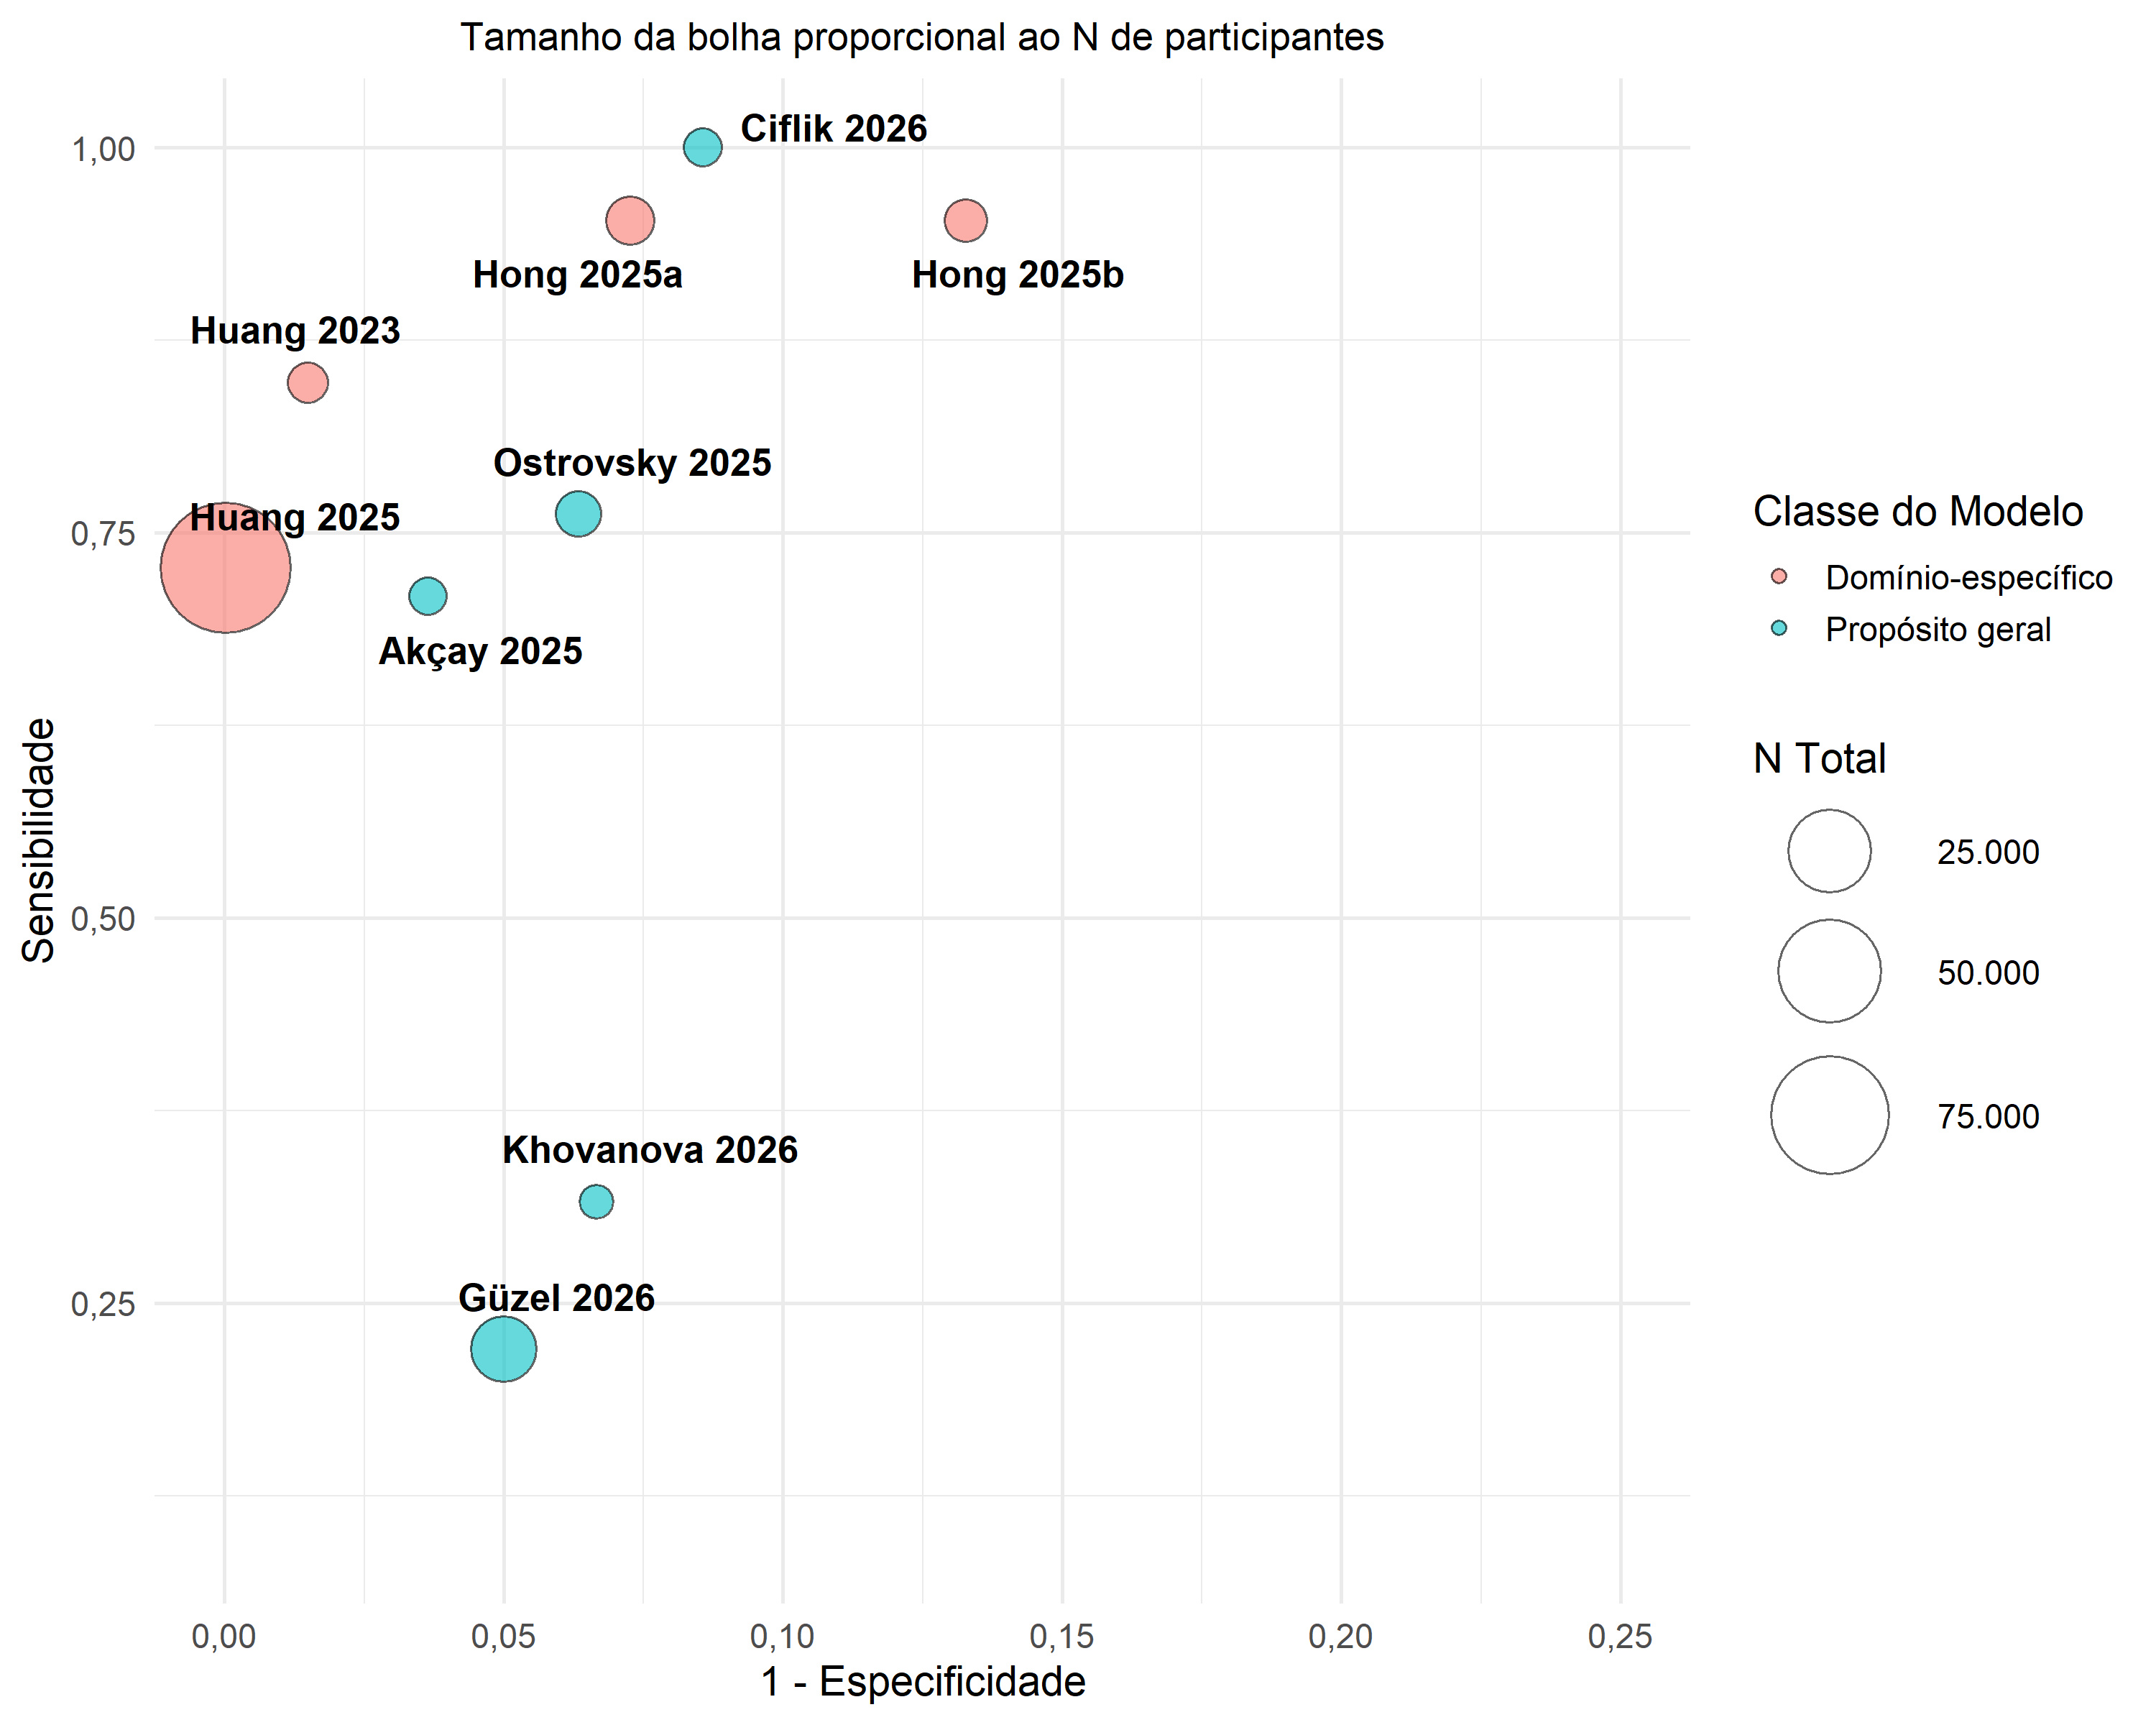
\includegraphics[width=0.85\textwidth]{figures/Fig6_BubblePlot_V10.jpg}
    \vspace{4pt}
    \begin{singlespace}
    \centering\small Fonte: Elaborado pelo autor (2026).
    \end{singlespace}
\end{figure}

\subsubsection{Por Condição Clínica}
O desempenho variou de forma acentuada conforme a patologia avaliada. O subgrupo de pneumotórax reúne 5 estudos (110.931 exames: Hong 2025a, Huang 2025, Akçay 2025, Ciflik 2026 e Güzel 2026) e as demais condições reúnem 4 estudos (2.783 exames: Hong 2025b, Ostrovsky 2025, Huang 2023 e Khovanova 2026). Para a detecção de tuberculose (Hong 2025b), a sensibilidade individual foi elevada (95,2\%, com especificidade de 86,7\%), refletindo o bom desempenho do modelo em identificar padrões consolidation e infiltrados típicos de triagem epidemiológica. Para pneumonia (Ostrovsky 2025), a sensibilidade foi de 76,2\% e especificidade de 93,7\%.\footnote{O subconjunto de 1.400 imagens do \textit{NIH Chest X-ray} utilizado por Ostrovsky 2025 abrange sete categorias patológicas (200 imagens cada). A matriz 2$\times$2 aqui adotada refere-se especificamente à tarefa de pneumonia (sensibilidade 76,2\%, especificidade 93,7\%, conforme a tabela do artigo); consequentemente, os casos classificados como ``negativos'' incluem imagens de outras patologias além de exames estritamente normais, e o total de positivos reconstruído (185) aproxima-se dos 200 exames rotulados como pneumonia.} O pior desempenho geral ocorreu na detecção de nódulos pulmonares (Khovanova 2026), no qual a sensibilidade caiu para apenas 31,6\%, evidenciando a extrema dificuldade das IAs generativas em identificar lesões nodulares pequenas e isoladas.

\subsubsection{Por Tamanho e Gravidade da Lesão}
A acurácia dos modelos generativos mostrou-se altamente dependente do tamanho físico da patologia. No estudo de Akçay 2025 \cite{akcay}, a área sob a curva (AUC) do ChatGPT-4o para diagnosticar pneumotórax caiu drasticamente de 0,894 em lesões classificadas como grandes (distância hilum-pleura $\ge 2$ cm) para apenas 0,439 em lesões pequenas ($< 2$ cm), indicando desempenho inferior ao acaso em patologias sutis. No estudo em larga escala de Güzel 2026 \cite{guzel} (N=10.675 CXRs), a baixíssima sensibilidade global do GPT-4o, Gemini 2 e Claude 4 (variando entre 16,0\% e 36,0\%) foi atribuída diretamente à incapacidade dos modelos de identificar pequenos focos de colapso pulmonar no conjunto de dados SIIM-ACR.

\subsubsection{Por Grupo Demográfico}
A avaliação de subgrupos demográficos evidenciou viés etário relevante. No estudo retrospectivo de Bulut 2025 \cite{bulut} avaliando o diagnóstico de pneumotórax em um hospital terciário, a acurácia dos três modelos avaliados (ChatGPT-4o, Gemini 2.0 e Claude 3.5) decaiu de forma vertiginosa no subgrupo pediátrico (idade $\le 12$ anos), registrando taxas de acurácia entre 12,5\% e 20,8\%, em comparação ao subgrupo de pacientes adultos (57,4\% a 69,6\%). Esta diferença decorre de fatores anatômicos específicos da infância (estruturas ósseas mais finas, timo proeminente e maior frequência de artefatos de choro/movimentação), para os quais os modelos genéricos não receberam treinamento adequado.

\subsection{Impacto no Fluxo de Trabalho (Workflow) Clínico}
A introdução de laudos estruturados preliminares gerados por IA foi associada a melhorias significativas de fluxo. No reader study multicêntrico de Hong 2025c \cite{hong2025c} (N=758 exames avaliados por 5 radiologistas), a assistência do modelo de IA específico (KARA-CXR) reduziu o tempo médio de interpretação e emissão de laudo de 34,2 segundos ($\pm 20,4$) para 19,8 segundos ($\pm 12,5$) por exame, representando um ganho de eficiência de aproximadamente 42\% ($P < 0,001$). A qualidade do relatório final manteve-se equivalente ou superior à leitura humana padrão. 

Além disso, a sensibilidade dos médicos em detectar condições desafiadoras aumentou significativamente com o suporte da IA: a sensibilidade para identificar lesões pleurais subiu de 77,7\% para 87,4\% ($P < 0,001$) e para alargamento de silhueta mediastinal aumentou de 84,3\% para 90,8\% ($P < 0,001$). A taxa de aceitação sem modificações (acceptability) do laudo gerado pela IA específica foi de 70,5\% para o modelo KARA-CXR (comparado a apenas 29,6\% para o GPT-4V de propósito geral), demonstrando que IAs customizadas possuem linguagem clínica superior e reduzem a sobrecarga de digitação do radiologista.

\subsection{Qualidade Textual e Alucinações nos Laudos Gerados}
Apesar dos benefícios de velocidade, os laudos gerados exibiram inconsistências descritivas e alucinações textuais. No estudo de Hong 2025b \cite{hong2025b} avaliando triagem de tuberculose, a taxa de erro de localização anatômica lateral da IA foi de 36,7\% (acurácia de localização de apenas 63,3\%), com o modelo gerando laudos que descreviam consolidações apicais no pulmão direito quando a lesão real localizava-se no pulmão esquerdo. Adicionalmente, em análises qualitativas de factualidade (como em ReXamine-Global \cite{banerjee}), os modelos apresentaram alucinações graves, como descrever fraturas costais e níveis hidroaéreos que não constavam nas imagens, ou citar a presença de um tubo endotraqueal bem posicionado em radiografias de pacientes que não estavam intubados.

\newpage
\section{DISCUSSÃO}

\subsection{Interpretação das Estimativas}
Os resultados da meta-análise apontam para especificidade agrupada elevada (96,8\%) acompanhada de sensibilidade apenas intermediária (78,1\%). Cabe ressaltar que nenhum dos estudos do pool principal comparou os modelos generativos ao desempenho de radiologistas sobre a mesma amostra; esta síntese, portanto, não autoriza qualquer afirmação de equivalência ou paridade diagnóstica com leitores humanos. Além disso, a elevada dispersão expressa no intervalo de predição [6,4\%; 99,5\%] indica que o ponto sumário não deve ser interpretado como uma garantia de desempenho estática --- tampouco como um parâmetro transferível a um contexto clínico específico. A grande variação decorre do desalinhamento de construto entre os estudos incluídos, nos quais as tarefas de diagnóstico variam desde a detecção simples de pneumotórax até a caracterização clínica complexa de infiltrados e nódulos pulmonares.

\subsection{Implicações da Dominância Amostral}
A análise de dominância amostral revelou que as altas estimativas de especificidade do pool completo são fortemente influenciadas pelo estudo prospectivo de Huang 2025 \cite{huang2025}, que contribui com 97.651 dos 113.714 participantes (85,9\% do peso meta-analítico).\footnote{O estudo de Huang 2025 não apresenta uma matriz 2$\times$2 única para o desfecho de pneumotórax. As células aqui empregadas foram reconstruídas a partir de duas sub-análises reportadas no artigo: a coorte de sensibilidade (33 pneumotórax inesperados que preencheram os critérios de priorização, dos quais 24 foram sinalizados, resultando em VP=24 e FN=9) e a coorte de precisão do sistema de sinalização (78 exames sinalizados, dos quais 56 verdadeiros, resultando em FP=22); os verdadeiros negativos (97.596) foram obtidos por complemento sobre os 97.651 exames rastreados. O par sensibilidade 72,7\%/especificidade 99,9\% corresponde ao resultado principal declarado pelos autores.} Como a prevalência de pneumotórax na coorte de Huang 2025 foi extremamente baixa (0,03\%, correspondendo a apenas 33 casos positivos em quase 100.000 exames), a especificidade de 100\% obtida pelo modelo influenciou pesadamente a estimativa agrupada. O Cenário B (sem Huang 2025), uma das cinco análises de sensibilidade pré-especificadas na Seção 2.7, recoloca a especificidade em 93,7\% e é adotado, nesta revisão, como o cenário de referência para leitura clínica e para eventuais projeções regulatórias, por remover a distorção de especificidade induzida pela prevalência extrema sem excluir o estudo de pior desempenho (Güzel 2026). A aplicação das razões de verossimilhança do ponto sumário a probabilidades pré-teste clinicamente plausíveis (Figura \ref{fig:fagan}) delimita essa utilidade de forma quantitativa: partindo de uma prevalência de 20\%, um resultado positivo eleva a probabilidade pós-teste para 85,8\%, ao passo que um resultado negativo a reduz apenas para 5,4\% --- patamar incompatível com a exclusão segura de pneumotórax agudo. Para prevalências de 10\% e 5\%, a probabilidade pós-teste negativa situa-se em 2,5\% e 1,2\%, respectivamente. Ou seja, mesmo em cenários de baixa prevalência, o desempenho observado sustenta melhor a confirmação do que a exclusão diagnóstica.

\begin{figure}[H]
    \centering
    \caption{Nomograma de Fagan: Probabilidades Pós-teste para Cenários Clínicos.}
    \label{fig:fagan}
    \vspace{4pt}
    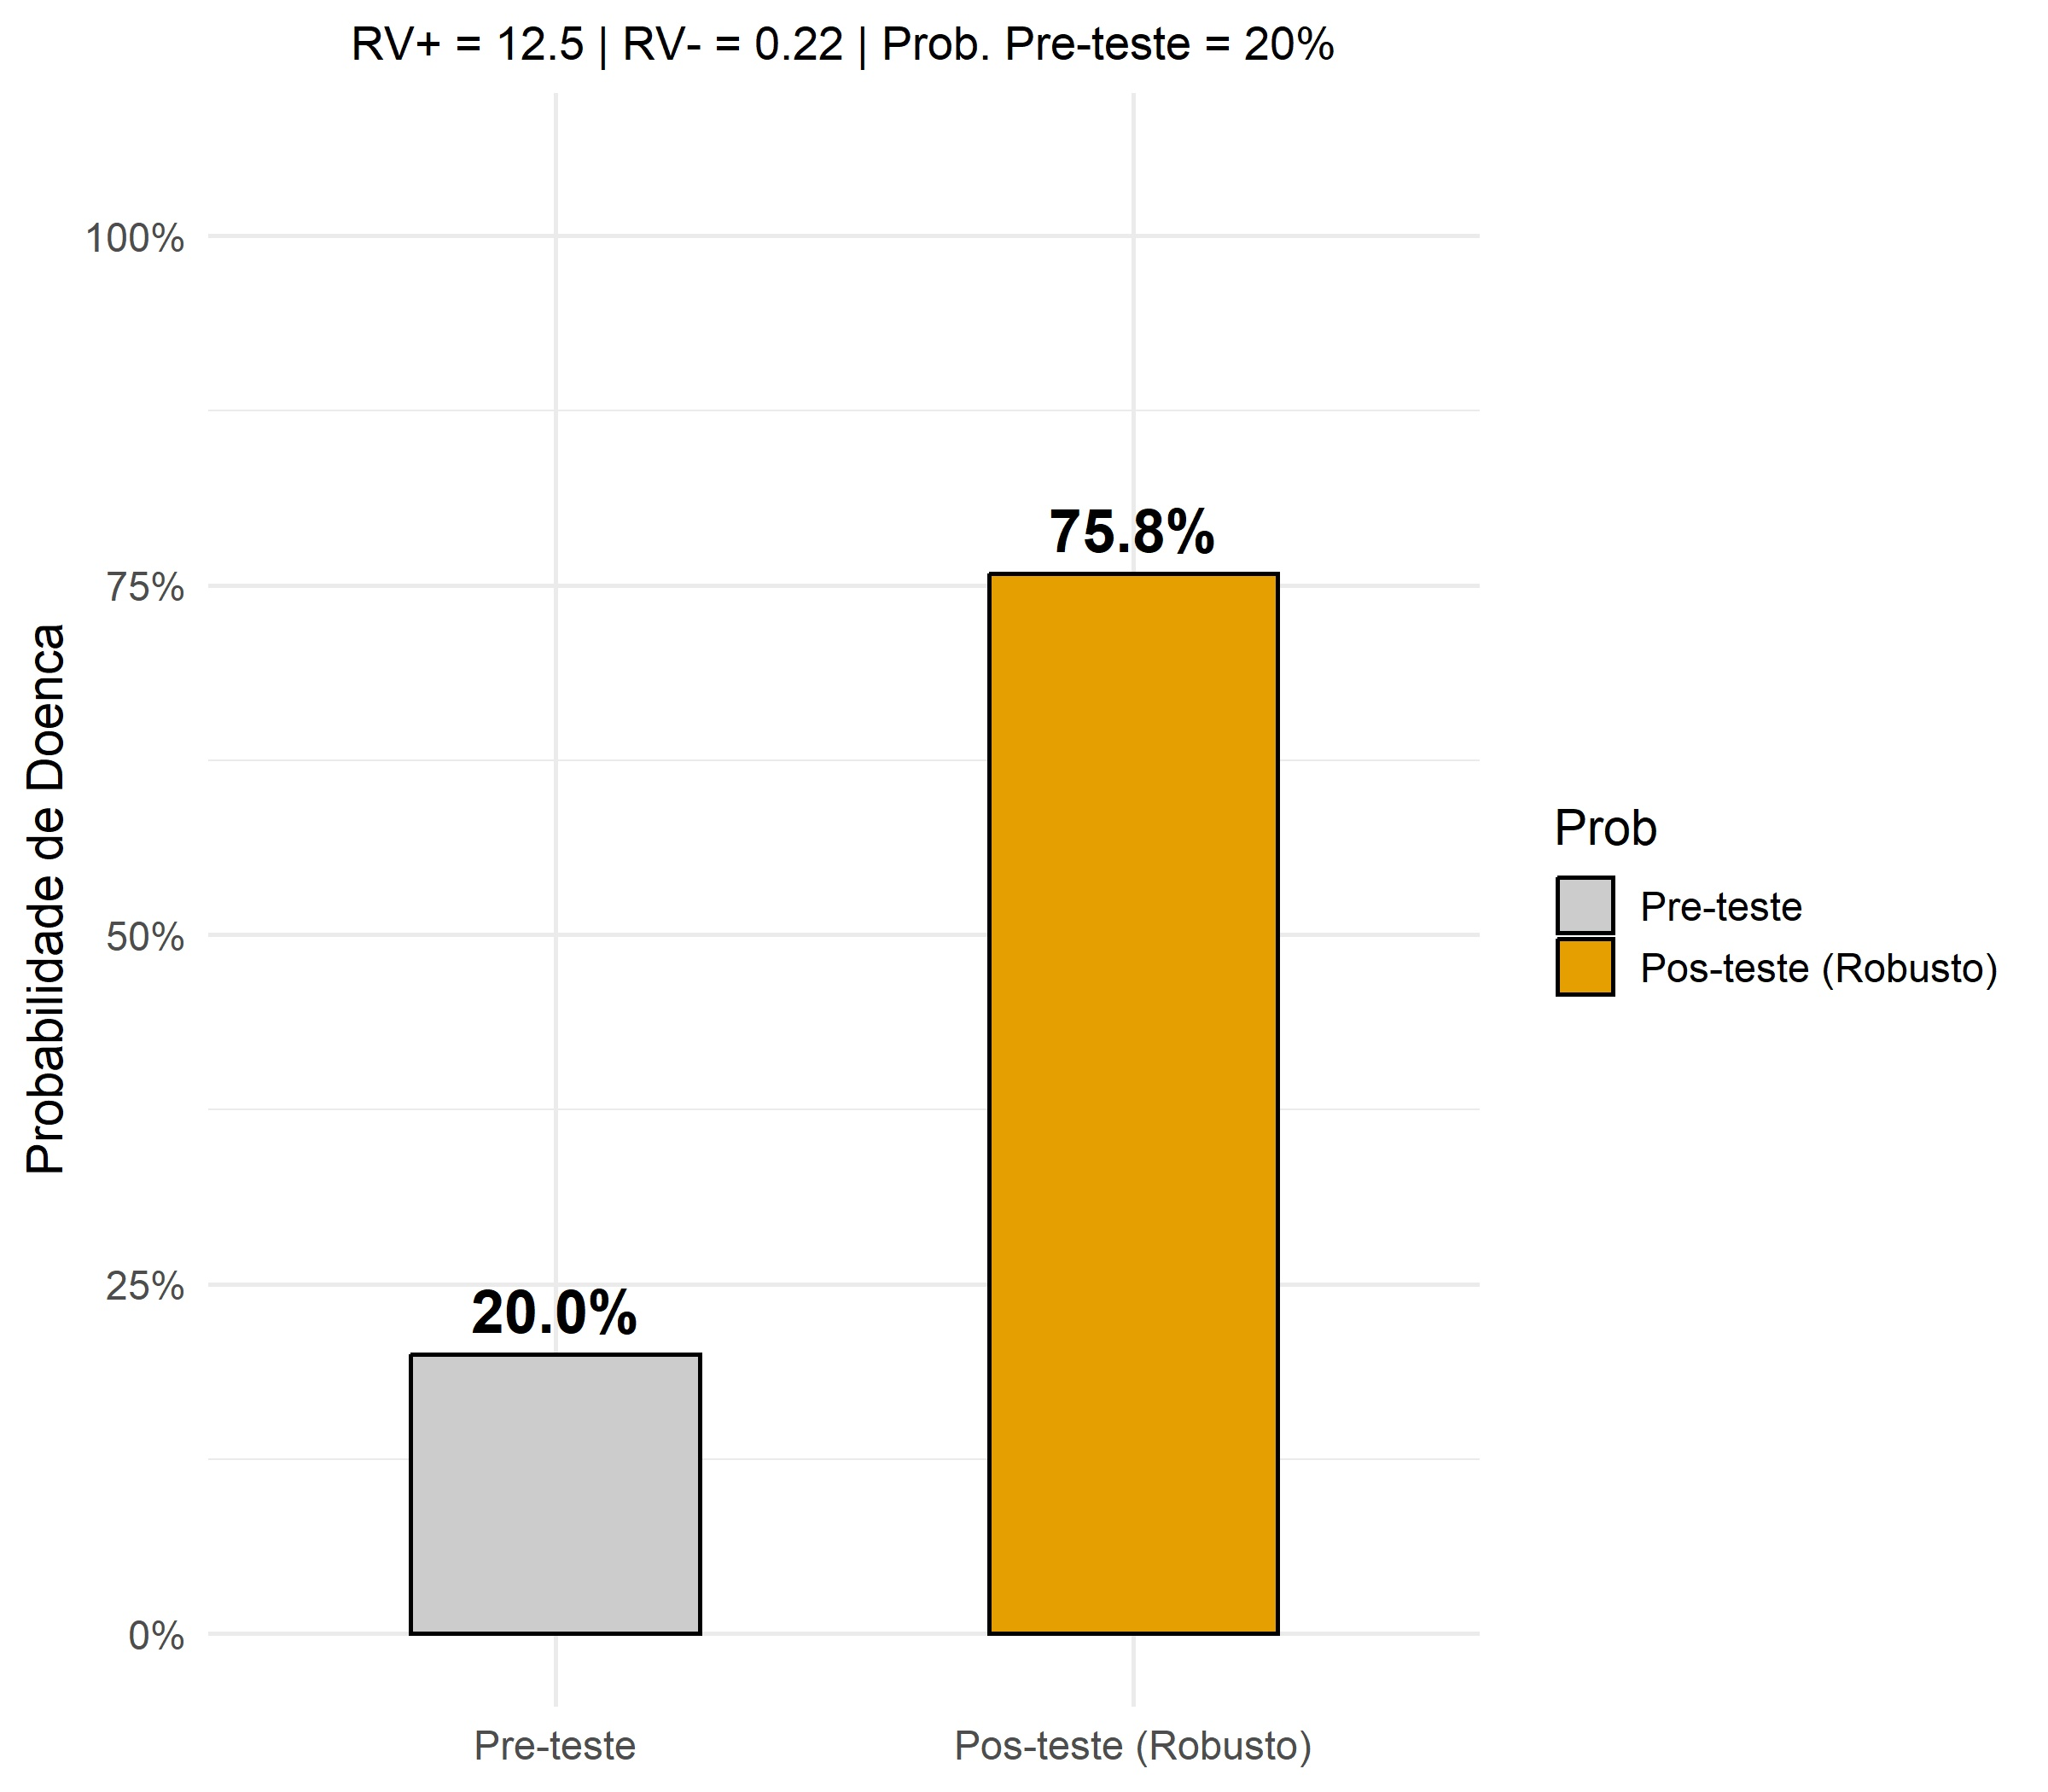
\includegraphics[width=0.85\textwidth]{figures/Fig3_Fagan_Robust_V10.jpg}
    \vspace{4pt}
    \begin{singlespace}
    \centering\small Fonte: Elaborado pelo autor (2026).
    \end{singlespace}
\end{figure}

\subsection{Perfis por Especialização do Modelo}
O contraste entre modelos domínio-específicos e de propósito geral concentra o achado exploratório mais consistente desta revisão: a especificidade média é praticamente idêntica nos dois grupos (94,5\% vs. 94,0\%), ao passo que a sensibilidade média cai de 87,0\% para 60,1\% nos modelos generalistas. Isso sugere que a adaptação ao domínio radiológico atua sobretudo sobre a capacidade de \textit{detecção} do achado, e não sobre a capacidade de descartar normalidade. Modelos treinados em laudos radiológicos reais parecem desenvolver representações mais sensíveis a achados sutis, enquanto modelos proprietários multiuso (GPT-4o, Gemini 2, Claude) aplicam limiares internos de decisão mais conservadores, resultando em menor sensibilidade diagnóstica sem ganho correspondente de especificidade. Reitera-se, contudo, que os dois braços diferem também quanto à tarefa e ao tamanho das lesões avaliadas, de modo que a especialização do modelo não pode ser isolada como causa única.

Esse comportamento conservador é especialmente evidente em modelos proprietários de propósito geral avaliados em conjuntos de dados desafiadores. No estudo de Güzel 2026 \cite{guzel}, a sensibilidade de modelos como Gemini 2 Pro e Claude 4 Sonnet para detecção de pneumotórax desabou para patamares entre 16,0\% e 36,0\% (com sensibilidade média de 22,0\%), enquanto a especificidade manteve-se consistentemente acima de 95,0\%. Um padrão semelhante foi documentado por Khovanova 2026 \cite{khovanova}, em que o Claude 3.7 Sonnet obteve sensibilidade de apenas 31,6\% na detecção de nódulos pulmonares. 

Este fenômeno pode ser explicado pelas restrições de segurança impostas durante o treinamento desses modelos comerciais por meio de Aprendizado por Reforço com Feedback Humano (RLHF). Para mitigar alucinações (geração de achados inexistentes ou falsos positivos), os desenvolvedores aplicam penalidades severas à geração de relatórios espúrios. Diante de qualquer incerteza visual em uma imagem sutil ou pouco conspícua, o modelo adota um threshold de decisão extremamente alto, preferindo classificar o exame como "dentro dos limites da normalidade" ou "sem alterações agudas". Embora essa estratégia minimize falsos alarmes (alta especificidade), ela induz uma taxa inaceitável de falsos negativos (baixa sensibilidade), limitando a utilidade desses sistemas como ferramentas autônomas de triagem médica.

\subsection{O Impacto da Engenharia de Prompts}
A formulação das instruções fornecidas às IAs generativas atua como o principal threshold de decisão clínica do sistema. Nos estudos incluídos, prompts instrucionais curtos que forçavam respostas binárias rígidas (como ``pneumotórax presente: 1 ou 0'', adotado em Güzel 2026 \cite{guzel} e Akçay 2025 \cite{akcay}) resultaram em taxas de sensibilidade sensivelmente inferiores às obtidas em estudos onde os prompts permitiam a geração de laudos em texto livre (como nos estudos de Hong 2025a/b). Adicionalmente, quando o prompt inclui o contexto clínico prévio (histórico de dor torácica ou suspeita de trauma), observa-se aumento de sensibilidade, pois o modelo de linguagem ancora sua atenção em regiões de maior probabilidade, de forma similar ao raciocínio diagnóstico de um radiologista humano.

\subsection{Ferramenta Diagnóstica Isolada vs. Colaboração Humano-IA}
A evidência cumulativa demonstra que os modelos multimodais de IA generativa não apresentam segurança científica para uso autônomo na prática clínica. A baixa sensibilidade demonstrada na detecção de lesões sutis (como nódulos pulmonares em Khovanova 2026 \cite{khovanova} ou pneumotórax pequeno em Akçay 2025 \cite{akcay}) inviabiliza o emprego dessas ferramentas como mecanismos de exclusão de diagnóstico (rule-out). O papel clinicamente seguro e suportado pelas evidências é o de segunda leitura assistida (copiloto). Nesse modelo de uso colaborativo, a IA funciona como um revisor preliminar que agiliza o laudo e previne omissões por fadiga visual do radiologista, mantendo a responsabilidade final do diagnóstico sob supervisão e validação humana obrigatória.

No entanto, a transição de modelos tradicionais de redes neurais convolucionais (CNNs) para modelos multimodais generativos introduz o chamado **gap de explicabilidade**. As CNNs clássicas de classificação visual costumam ser acompanhadas por mapas de calor baseados em ativação (como o Grad-CAM), os quais fornecem uma explicabilidade espacial direta ao apontar a região exata do pixel que determinou a inferência da IA. Em contrapartida, as IAs generativas produzem laudos textuais fluentes em linguagem livre que descrevem a patologia de forma descritiva, mas carecem de mecanismos nativos de ancoragem espacial visual (*grounding*). Essa lacuna dá origem a um tipo inédito de erro na radiologia computadorizada: o **diagnóstico correto com atribuição espacial incorreta**. Como observado no estudo de triagem de tuberculose de Hong 2025b \cite{hong2025b}, a IA gerou laudos descrevendo consolidações no pulmão direito quando a lesão real localizava-se no pulmão esquerdo, registrando uma taxa de erro de lateralidade de 36,7\%. Esse descompasso semântico-visual exige que o radiologista humano atue não apenas validando a presença da patologia sugerida, mas auditando meticulosamente a coerência espacial descrita pelo modelo.

Adicionalmente, os ganhos expressivos de eficiência no fluxo de trabalho clínico --- como a redução de 42\% no tempo de digitação e leitura documentada por Hong 2025c \cite{hong2025c} --- trazem consigo o risco latente do **viés de automação** associado à fadiga cognitiva. Sob condições de sobrecarga crônica de trabalho e exaustão mental (conforme discutido na Seção 1.1), o radiologista tende a aceitar passivamente o laudo preliminar gerado pela IA para acelerar a liberação do exame, reduzindo seu nível de escrutínio ativo sobre a imagem. Evidência longitudinal corrobora essa preocupação: no estudo multileitor longitudinal de Hong et al. \cite{hongjacr} (756 radiografias interpretadas por cinco radiologistas em sete lotes sequenciais ao longo de um mês) --- publicação distinta do \textit{reader study} de Hong 2025c \cite{hong2025c}, embora oriunda do mesmo grupo e do mesmo sistema de IA ---, a taxa de aceitação dos laudos de IA sem modificação aumentou progressivamente de 54,6\% para 60,2\% ($P < 0,001$) à medida que os leitores se habituavam à ferramenta, enquanto a concordância e a qualidade permaneceram estáveis nos exames normais mas oscilaram nos casos anormais --- justamente os que mais demandam escrutínio independente. Esse comportamento passivo pode induzir o fenômeno de **co-omissão**: caso a IA generativa falhe em relatar um achado sutil ou pequeno (cenário frequente devido ao gargalo de compressão de 8 bits), o radiologista, induzido pelo relatório "normal" da IA, também deixará de detectar a patologia. Assim, a colaboração Humano-IA só se traduz em incremento real de segurança se houver salvaguardas de fluxo que forcem o médico a realizar uma leitura visual independente antes de visualizar a sugestão textual da máquina, mitigando a transferência sistemática dos erros do algoritmo para o diagnóstico do paciente.

\subsection{Lacunas da Literatura Primária}
A literatura primária apresenta lacunas estruturais significativas que limitam o alcance das sínteses quantitativas atuais. Em primeiro lugar, destaca-se o **gargalo de compressão e resolução da imagem**. A radiologia digital utiliza nativamente arquivos no padrão DICOM (*Digital Imaging and Communications in Medicine*), que possuem profundidades de cor variando de 12 a 16 bits, o que corresponde a uma escala de cinza com 4.096 a 65.536 níveis de intensidade. Além disso, a prática radiológica humana baseia-se no ajuste interativo de brilho e contraste (*windowing* ou janelamento) no monitor diagnóstico, permitindo ao médico realçar linhas pleurais sutis ou pequenas atenuações nodulares pulmonares. 

Entre os estudos primários que descreveram explicitamente o pré-processamento de imagem, a conversão do DICOM original para formatos de 8 bits (JPEG ou PNG) --- que oferecem apenas 256 níveis de cinza --- foi a prática predominante, documentada em Güzel 2026 \cite{guzel} (que detalha um fluxo explícito de conversão DICOM para PNG de 8 bits), Khovanova 2026 \cite{khovanova}, Akçay 2025 \cite{akcay}, Ciflik 2026 \cite{ciflik} e Hong 2025a \cite{hong2025a}, frequentemente acompanhada de redimensionamento para resoluções reduzidas (da ordem de 224$\times$224 a 1.024$\times$1.024 pixels), de modo a atender às limitações computacionais dos codificadores visuais. Registre-se, todavia, que parcela relevante dos estudos incluídos \textbf{não relata} o formato de arquivo nem a profundidade de bits das imagens submetidas ao modelo --- omissão que, por si só, constitui lacuna de reporte e impede quantificar com precisão o alcance desse gargalo. Esta compressão e perda de profundidade de bits causam uma **destruição física de informações de alta frequência espacial**, eliminando o contraste tênue necessário para visualizar descolamentos pleurais finos (como no pneumotórax sutil) ou densidades de tecidos moles pequenas (nódulos menores que 1 cm). Esse fator explica por que o desempenho da IA decaiu de forma tão acentuada para lesões pequenas nos estudos de Akçay 2025 \cite{akcay} e Güzel 2026 \cite{guzel}, revelando que a baixa acurácia em patologias sutis é, em grande parte, uma limitação física da qualidade da imagem de entrada fornecida ao modelo, e não apenas um déficit cognitivo de interpretação.

Em segundo lugar, observa-se uma quase total ausência de dados clínicos estruturados e integrados (sintomas, dados laboratoriais) nos conjuntos de teste primários, forçando os modelos a realizar leituras visuais cegas desprovidas de contexto. Na prática clínica, o histórico do paciente (ex: "tabagista pesado com tosse produtiva" ou "pós-procedimento de acesso venoso central") atua como um prior bayesiano que orienta a busca visual do radiologista; a privação desse contexto penaliza injustamente os modelos generativos.

Por fim, a falta de publicação das matrizes de confusão completas e dos logs de prompt em repositórios públicos (como observado em Lee 2025 \cite{lee} e Bulut 2025 \cite{bulut}) impede a reprodutibilidade dos resultados. Trabalhos recentes de alto impacto publicados em periódicos como \textit{Nature Communications} (Bai et al. 2026 \cite{bai}, propondo o framework Janus-Pro-CXR baseado no backbone DeepSeek) começam a introduzir o reporte padronizado de curvas ROC e áreas sob a curva por achado específico, mas ainda há escassez de matrizes 2$\times$2 brutas.

\subsection{Limitações}
As limitações deste estudo meta-analítico incluem:
\begin{enumerate}
    \item Processo de revisor único nas etapas de julgamento: embora a triagem de títulos e resumos tenha sido automatizada e determinística (TF-IDF), a avaliação de elegibilidade por texto completo, a extração das matrizes de contingência 2$\times$2 e o julgamento QUADAS-2 foram conduzidos por um único revisor. A ausência de um segundo revisor independente e cego impede o cálculo da concordância interavaliador (kappa de Cohen) e expõe essas etapas a viés de seleção e de extração, constituindo a principal limitação metodológica desta revisão; a replicação independente requer a incorporação de um segundo avaliador;
    \item Dominância amostral extrema do estudo Huang 2025, condicionando a especificidade agrupada;
    \item Intervalo de predição de sensibilidade muito amplo, limitando a generalização do ponto sumário;
    \item Viés de independência estatística pelo uso de dados originados do mesmo grupo e sistema (cluster Hong 2025a/b, com Hong 2025c e o reader study longitudinal de Hong et al. \cite{hongjacr} reforçando a dependência entre publicações do mesmo grupo);
    \item Poucos estudos no subgrupo de LLM puro (N=2), impedindo testes formais de heterogeneidade por arquitetura;
    \item Cobertura geográfica restrita a exames de instituições dos Estados Unidos, Coreia do Sul, Turquia e Rússia, reduzindo a validade externa para populações da América Latina;
    \item Avaliação retrospectiva predominante nos estudos bivariados incluídos.
\end{enumerate}

\subsection{Implicações Regulatórias e Governança}
No cenário regulatório brasileiro, sistemas de auxílio diagnóstico baseados em inteligência artificial são classificados como Software como Dispositivo Médico (SaMD) e estão sujeitos à regulação sanitária da ANVISA, sob as diretrizes da RDC 657/2022. Sob esta resolução, as ferramentas de IA generativa e multimodal necessitam de validação clínica retrospectiva e prospectiva multicêntrica em dados nacionais antes de serem aprovadas para fins comerciais e assistenciais. A ausência de validação em exames de pacientes do sistema público de saúde brasileiro (SUS) e as frequentes alucinações descritas reforçam que, sob as normas da ANVISA, esses sistemas não reúnem os requisitos necessários para uso autônomo, sendo sua indicação de uso obrigatoriamente restrita a ferramentas de apoio diagnóstico com revisão humana compulsória.

\newpage
\section{CONCLUSÃO}
A presente revisão sistemática avaliou a acurácia diagnóstica de modelos de IA generativa e multimodal na interpretação de radiografias de tórax. O pool principal de N=9 estudos, totalizando 113.714 participantes, estimou sensibilidade agrupada de 78,1\% e especificidade agrupada de 96,8\%; a especificidade é condicionada pela dominância de um único estudo prospectivo de baixíssima prevalência (Huang 2025), ajustando-se para 93,7\% no cenário de referência (sem esse estudo). Cumpre enfatizar, contudo, que esse ponto sumário tem valor exploratório e não deve ser tomado como parâmetro de desempenho transferível: ele agrega condições-alvo heterogêneas (pneumotórax, tuberculose, pneumonia e nódulo pulmonar) que não configuram um estimando clínico único, e o intervalo de predição de 6,4\% a 99,5\% para a sensibilidade indica que o valor agrupado não prediz de forma útil o desempenho em um novo cenário.

A contribuição mais robusta desta revisão não reside, portanto, na estimativa agrupada, mas em dois achados convergentes e consistentes entre estudos independentes. O primeiro é o colapso da sensibilidade diante de lesões pequenas e pouco conspícuas --- 22,0\% em Güzel 2026, 31,6\% em Khovanova 2026 e AUC de 0,439 para pneumotórax menor que 2 cm em Akçay 2025 ---, padrão que sustenta com segurança a recusa do uso autônomo para exclusão diagnóstica. O segundo é a diferença sistemática entre modelos adaptados ao domínio radiológico e modelos comerciais de propósito geral, cuja sensibilidade média cai de 87,0\% para 60,1\% sem ganho correspondente de especificidade.

Recomenda-se a adoção de um padrão mínimo de reporte metodológico em estudos futuros (framework PIRT-IA), contemplando a disponibilização de matrizes 2$\times$2 completas por threshold avaliado, descrição do prompt e temperatura de inferência, especificação do formato de imagem (DICOM vs. PNG) e a presença de controle clínico de alucinações. O uso clínico desses modelos generativos mostra-se inviável de forma autônoma ou para fins de exclusão rápida (rule-out) de patologias agudas devido à baixa sensibilidade diagnóstica demonstrada para lesões sutis e pequenas. Contudo, seu papel assistencial como segunda leitura acoplada à revisão humana obrigatória apresenta robustez estatística e científica, proporcionando redução no tempo de emissão de laudos e mitigação de erros por fadiga nos serviços de radiologia. Ressalta-se, todavia, que a evidência longitudinal de aumento progressivo da aceitação passiva dos laudos gerados por IA à medida que os radiologistas se habituam à ferramenta reforça a necessidade de salvaguardas de fluxo que preservem a leitura visual independente, sob pena de transferência sistemática dos erros do modelo para o diagnóstico final.

\newpage
\begin{thebibliography}{99}

\bibitem{vanginneken} VAN GINNEKEN, B. Fifty years of computer analysis in chest imaging: rule-based, machine learning, deep learning. \textit{Radiological Physics and Technology}, v. 10, n. 1, p. 23--32, 2017.

\bibitem{parikh} PARIKH, J. R.; VAN MOORE, A.; MEAD, L. et al. Prevalence of burnout of radiologists in private practice. \textit{Journal of the American College of Radiology}, v. 20, n. 7, p. 712--718, 2023.

\bibitem{ostrovsky} OSTROVSKY, A. M. Evaluating a large language model's accuracy in chest X-ray interpretation for acute thoracic conditions. \textit{American Journal of Emergency Medicine}, v. 93, p. 99--102, 2025.

\bibitem{mcinnes} MCINNES, M. D. F.; MOHER, D.; THOMBS, B. D. et al. Preferred Reporting Items for a Systematic Review and Meta-analysis of Diagnostic Test Accuracy Studies: The PRISMA-DTA Statement. \textit{JAMA}, v. 319, n. 4, p. 388--396, 2018.

\bibitem{whiting} WHITING, P. F.; RUTJES, A. W. S.; WESTWOOD, M. E. et al. QUADAS-2: a revised tool for the quality assessment of diagnostic accuracy studies. \textit{Annals of Internal Medicine}, v. 155, n. 8, p. 529--536, 2011.

\bibitem{stard} BOSSUYT, P. M.; REITSMA, J. B.; BRUNS, D. E. et al. STARD 2015: an updated list of essential items for reporting diagnostic accuracy studies. \textit{BMJ}, v. 351, p. h5527, 2015.

\bibitem{kagiyama} KAGIYAMA, N. et al. PRIME 2.0: Proposed Requirements for Cardiovascular Imaging-Related Multimodal AI Evaluation. \textit{JACC: Cardiovascular Imaging}, v. 19, n. 2, p. 223--251, 2026.

\bibitem{reitsma} REITSMA, J. B.; GLAS, A. S.; RUTJES, A. W. S. et al. Bivariate analysis of sensitivity and specificity produces informative summary measures in diagnostic reviews. \textit{Journal of Clinical Epidemiology}, v. 58, n. 10, p. 982--990, 2005.

\bibitem{ciflik} CIFLIK, K. B.; OZDEMIR CIFLIK, B. Evaluation of multimodal large language models for pneumothorax assessment in real-world clinical scenarios. \textit{BMC Pulmonary Medicine}, v. 26, n. 1, p. 105, 2026.

\bibitem{takwoingi} TAKWOINGI, Y.; GUO, B.; RILEY, R. D.; DEEKS, J. J. Performance of methods for meta-analysis of diagnostic test accuracy with few studies or sparse data. \textit{Statistical Methods in Medical Research}, v. 26, n. 4, p. 1896--1911, 2017.

\bibitem{guzel} GÜZEL, H. E.; ÖZENBA\c{S}, C.; KOÇ, A. M. Large-scale evaluation of multimodal large language models for pneumothorax detection. \textit{Diagnostic and Interventional Radiology}, 2026. doi:10.4274/dir.2026.263696.

\bibitem{huang2025} HUANG, J.; MOOR, M.; BANERJEE, O. et al. Efficiency and Quality of Generative AI-Assisted Radiograph Reporting. \textit{JAMA Network Open}, v. 8, n. 6, p. e2513921, 2025.

\bibitem{akcay} AKÇAY, O.; ÖZTÜRK, Ö. Evaluation of the effectiveness of the ChatGPT artificial intelligence application in the diagnosis of spontaneous pneumothorax on chest radiograph interpretation. \textit{BMC Pulmonary Medicine}, v. 26, n. 1, p. 8, 2025.

\bibitem{khovanova} KHOVANOVA, D.; VASILEV, Y.; VLADZYMYRSKYY, A. et al. A comparative accuracy study of multimodal LLMs, VLM and agent-based framework for pulmonary nodule detection on chest radiographs. \textit{Frontiers in Digital Health}, v. 7, p. 1674835, 2026.

\bibitem{lee} LEE, S.; YOUN, J.; KIM, H. et al. CXR-LLaVA: a multimodal large language model for interpreting chest X-ray images. \textit{European Radiology}, v. 35, n. 6, p. 4374--4386, 2025.

\bibitem{bai} BAI, Y.; ZHANG, R.; LEI, Y. et al. A DeepSeek-powered AI system for automated chest radiograph interpretation in clinical practice. \textit{Nature Communications}, 2026. No prelo. doi:10.1038/s41467-026-72680-6.

\bibitem{bulut} BULUT, B.; ÖZ, M. A.; GENÇ, M. et al. New frontiers in radiologic interpretation: Evaluating the effectiveness of large language models in pneumothorax diagnosis. \textit{PLoS ONE}, v. 20, n. 9, p. e0331962, 2025.

\bibitem{hong2025a} HONG, E. K.; HAM, J.; ROH, B. et al. Diagnostic Accuracy and Clinical Value of a Domain-specific Multimodal Generative AI Model for Chest Radiograph Report Generation. \textit{Radiology}, v. 314, n. 3, p. e241476, 2025.

\bibitem{hong2025b} HONG, E. K.; KIM, H. W.; SONG, O. K. et al. Multimodal Generative Artificial Intelligence Model for Creating Radiology Reports for Chest Radiographs in Patients Undergoing Tuberculosis Screening. \textit{American Journal of Roentgenology}, v. 225, n. 4, p. e2533059, 2025.

\bibitem{huang2023} HUANG, J.; NEILL, L.; WITTBRODT, M. et al. Generative Artificial Intelligence for Chest Radiograph Interpretation in the Emergency Department. \textit{JAMA Network Open}, v. 6, n. 10, p. e2336100, 2023.

\bibitem{hong2025c} HONG, E. K.; ROH, B.; PARK, B. et al. Value of Using a Generative AI Model in Chest Radiography Reporting: A Reader Study. \textit{Radiology}, v. 314, n. 3, p. e241646, 2025.

\bibitem{banerjee} BANERJEE, O.; SAENZ, A.; WU, K. et al. ReXamine-Global: A Framework for Uncovering Inconsistencies in Radiology Report Generation Metrics. \textit{arXiv preprint arXiv:2509.01188}, 2025.

\bibitem{hongjacr} HONG, E. K.; SUH, C. H.; NUKALA, M. et al. Radiologist Interaction with Artificial Intelligence-Generated Preliminary Reports: A Longitudinal Multireader Study. \textit{Journal of the American College of Radiology}, v. 23, n. 2, p. 292--298, 2026.
\end{thebibliography}

\end{document}
